%!TEX root = jt-thesis-main.tex

\section*{English Abstract}
\begin{onehalfspace}
	
	The english abstract is required for all english theses at TU-Berlin.
\end{onehalfspace}
\clearpage

\section*{Deutscher Abstract}
\begin{onehalfspace}
	
	Ein deutscher Abstract wird immer benötigt, für alle Abschlussarbeiten an
	der TU-Berlin. 
\end{onehalfspace}
\clearpage


\section{Introduction}
\label{sec:Introduction}
Gartner Inc. states that the number of network connected devices will reach
20.4 billion by 2020~\cite{gartner} To gather information from those devices,
we need algorithms which efficiently sample and route data from sensor nodes
(i.e., devices) to data sinks. Energy expenditure will gain higher importance,
especially for mobile devices such as battery-powered wearables and
smartphones. A \ac{WSN} is often battery-powered and use cases span from home
and health applications to the military sector~\cite{akyildiz2002wireless}.
With low production costs of a node as a goal in
\acp{WSN}~\cite{akyildiz2002wireless}, resource usage at the nodes is
restricted. While reducing sampling frequencies leads to a higher life of a
battery-powered sensor network, important changes in the observed phenomenon
could be missed which reduces the quality of the
data~\cite{akyildiz2002wireless}. A tradeoff between the quality of data and
energy expenditure arises, thus an optimization is needed. 
\par
Different methods for optimizing \acp{WSN} were presented in surveys
(e.g.,~\cite{abbasi2007survey, sivrikaya2004time, carrano2014survey}). The
proposed areas of optimization include clustering
algorithms~\cite{abbasi2007survey}, time
synchronization~\cite{sivrikaya2004time}, duty
cycling~\cite{carrano2014survey}, topology control~\cite{li2013survey},
in-network aggregation~\cite{fasolo2007network}, data
compression~\cite{srisooksai2012practical}, and general routing
techniques~\cite{al2004routing, kulkarni2011particle, singh2015survey,
rault2014energy}. Systems such as TinyDB~\cite{madden2005tinydb},
ACQUIRE~\cite{sadagopan2003acquire} and COUGAR~\cite{yao2002cougar} introduce
architectures for query processing in \acp{SN} which consist of algorithms for
sampling, and routing data requested by a user.

% TODO Expand Section with other subjects than wsns and energy conservation

\subsection{Motivation}
\label{sec:motivation}

As stated above, surveys and taxonomies were presented for different areas of
sensor networks. However, during our research, we did not encounter a survey or
catalog focusing on sampling algorithms in sensor data. This thesis provides a
catalog for a comprehensive overview of the existing sampling algorithms for
sensor data. For researchers as well as practitioners, a collection of sampling
algorithms is a valuable starting point for finding an algorithm suitable for a
specific usecase. Therefore, we present a taxonomy of the algorithms to provide
a compact overview. Furthermore, algorithms which focus on areas other than
sampling (like routing and topology control) in sensor networks will be
presented. Combinations of sampling, routing and topology control algorithms as
well as combinations of sampling algorithms from different categories can
inspire further research.


\subsection{Scientific Background}
\label{sec:Scientific Background}

Different types of \acp{SN}, like \acp{WSN}, \acp{RSN}, or wired \acp{SN}
exist. While all of them are used to monitor a phenomenon, like the temperature
in a room~\cite{labdata} or the behaviour of
wildlife~\cite{bennett2011cranetracker}, performance indicators vary in their
significance. Intuitively, wired \acp{SN} do not consider energy expenditure as
the primary concern. \acp{RSN} have a way to collect energy from the
environment they are stationed at, through, e.g. solar and wind or more exotic
variants like vibration~\cite{perpetuum}. To enable perpetual data collection
in \acp{RSN}, techniques for allocating sensing tasks to sensors while handling
the non linear emission of, e.g. solar and wind is
crucial~\cite{liu2011perpetual}. \acp{WSN} often have a limited energy source
at their disposal, making management of energy expenditure a top priority to
increase network lifetime. As Cheng et al. state~\cite{cheng2013stcdg} network
lifetime is often defined in \acp{WSN} as the lifetime of the first node to run
out of energy. 
\par
\acp{WSN} and \acp{RSN} are often designed with some nodes sensing the
phenomenon and one or more sink nodes wich transfer the sensed data to a
central base station. Based on the type of topology, e.g. a simple star
structure (Fig.~\ref{fig:Star Topology}), sensed data is forwarded to the sink
node directly, i.e. in a one-hop manner. More complex topologies, e.g. tree
(Fig.~\ref{fig:Tree Topology}) or connected star structures, often require to
relay sensed data through intermediary nodes to a sink node in a multi-hop
fashion, as direct communication paths between sensing and sink nodes are not
always possible~\cite{romer2004design}. 
\par
In more complex topologies with a lot of intermediary nodes, finding the
optimal routing path from sensor node to the sink is not trivial. With
increasing number of nodes, the complexity of the computation of the optimal
route increases, as nodes have multiple neighbors from which to choose the next
transmission step. Solving such a problem locally, i.e. nodes compute the next
best step, with additional contraints, e.g. minimizing energy expenditure and
meet quality of data thresholds can be an unfeasible task. On the other hand,
outsourcing this task to the base station could induce a major communication
overhead with additional energy expenditure. Techniques on topology control
and route path finding will be discussed later in the thesis.

% \begin{figure}
% \centering
% \begin{minipage}{.5\textwidth}
%   \centering
%   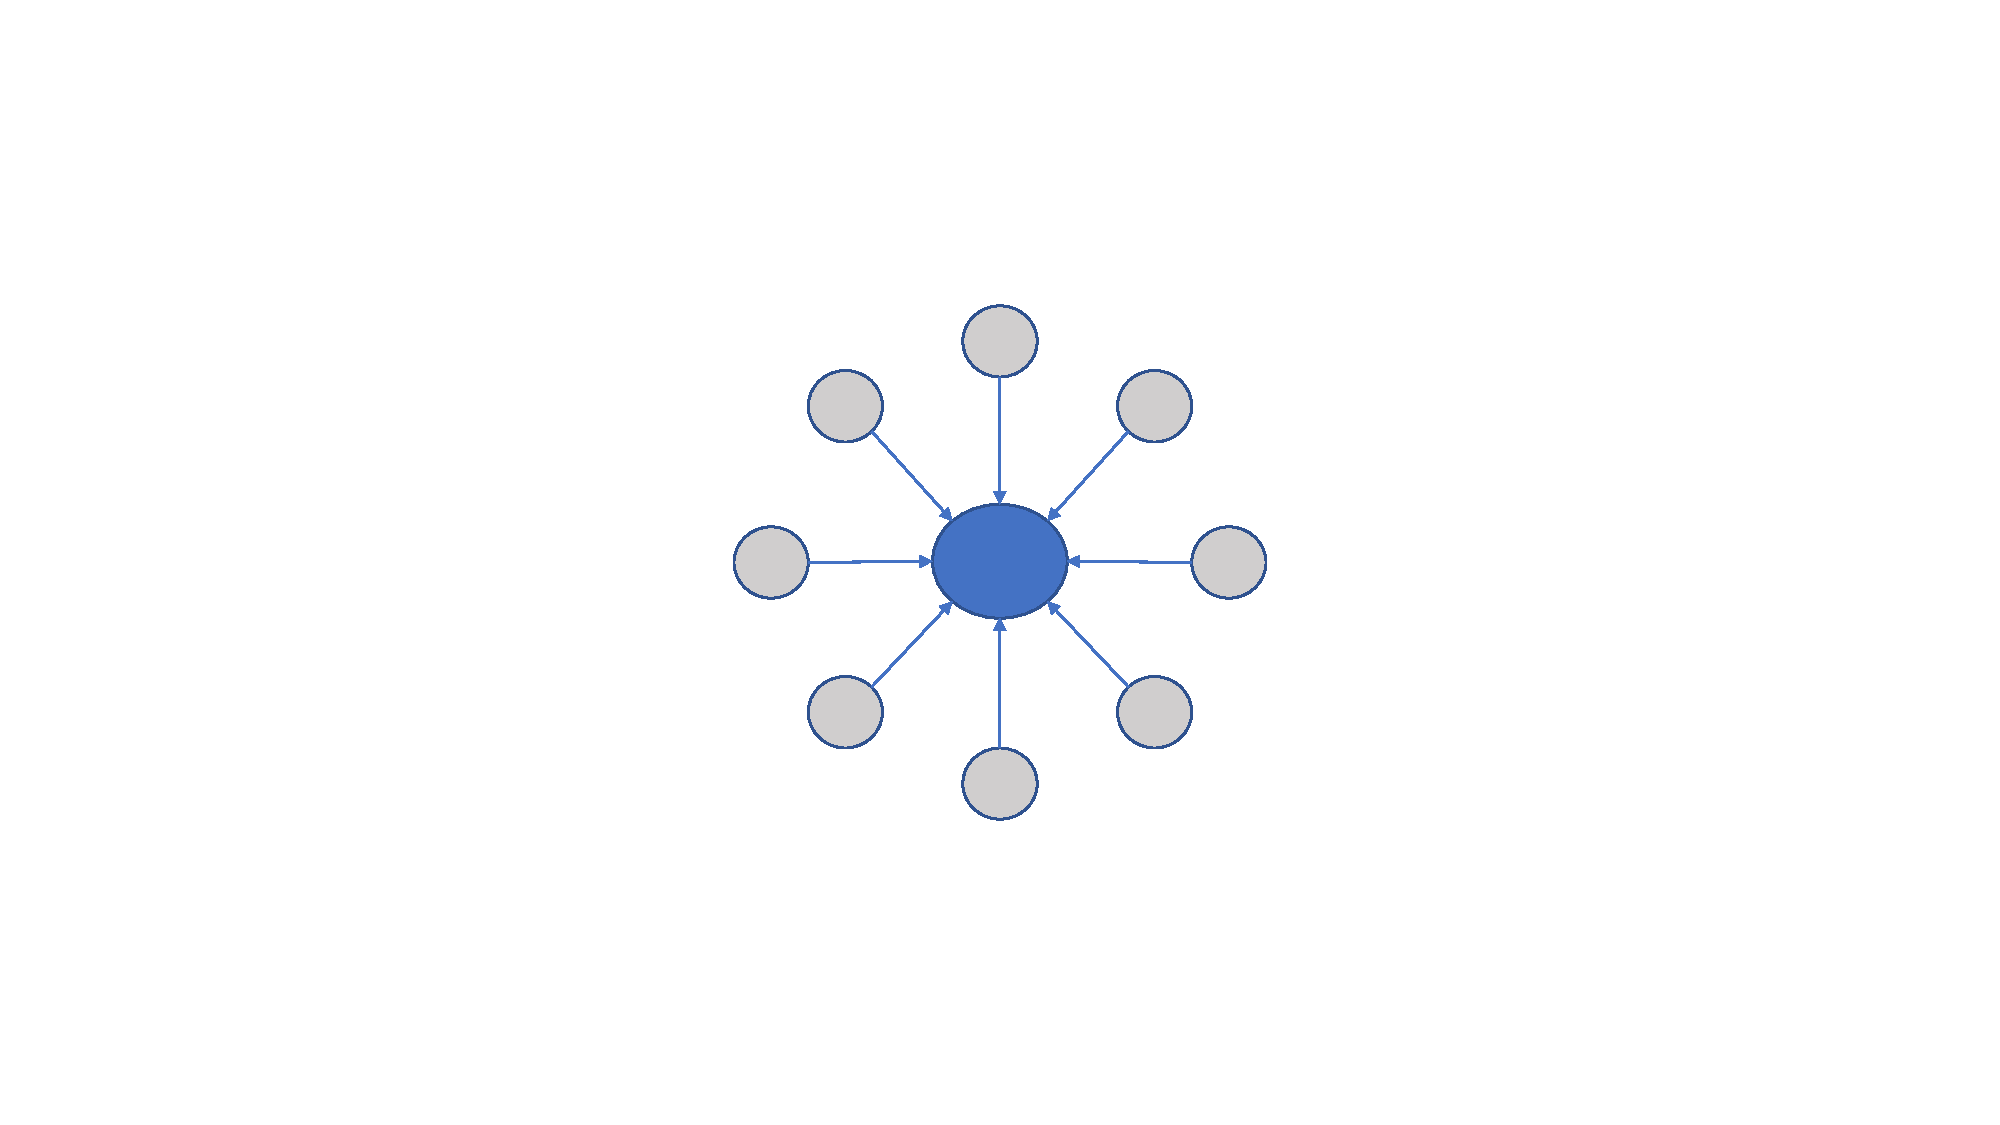
\includegraphics[width=\linewidth]{images/star-structure.pdf}
%   \caption{(a)}
%   \label{fig:Star Topology}
% \end{minipage}%
% \begin{minipage}{.5\textwidth}
%   \centering
%   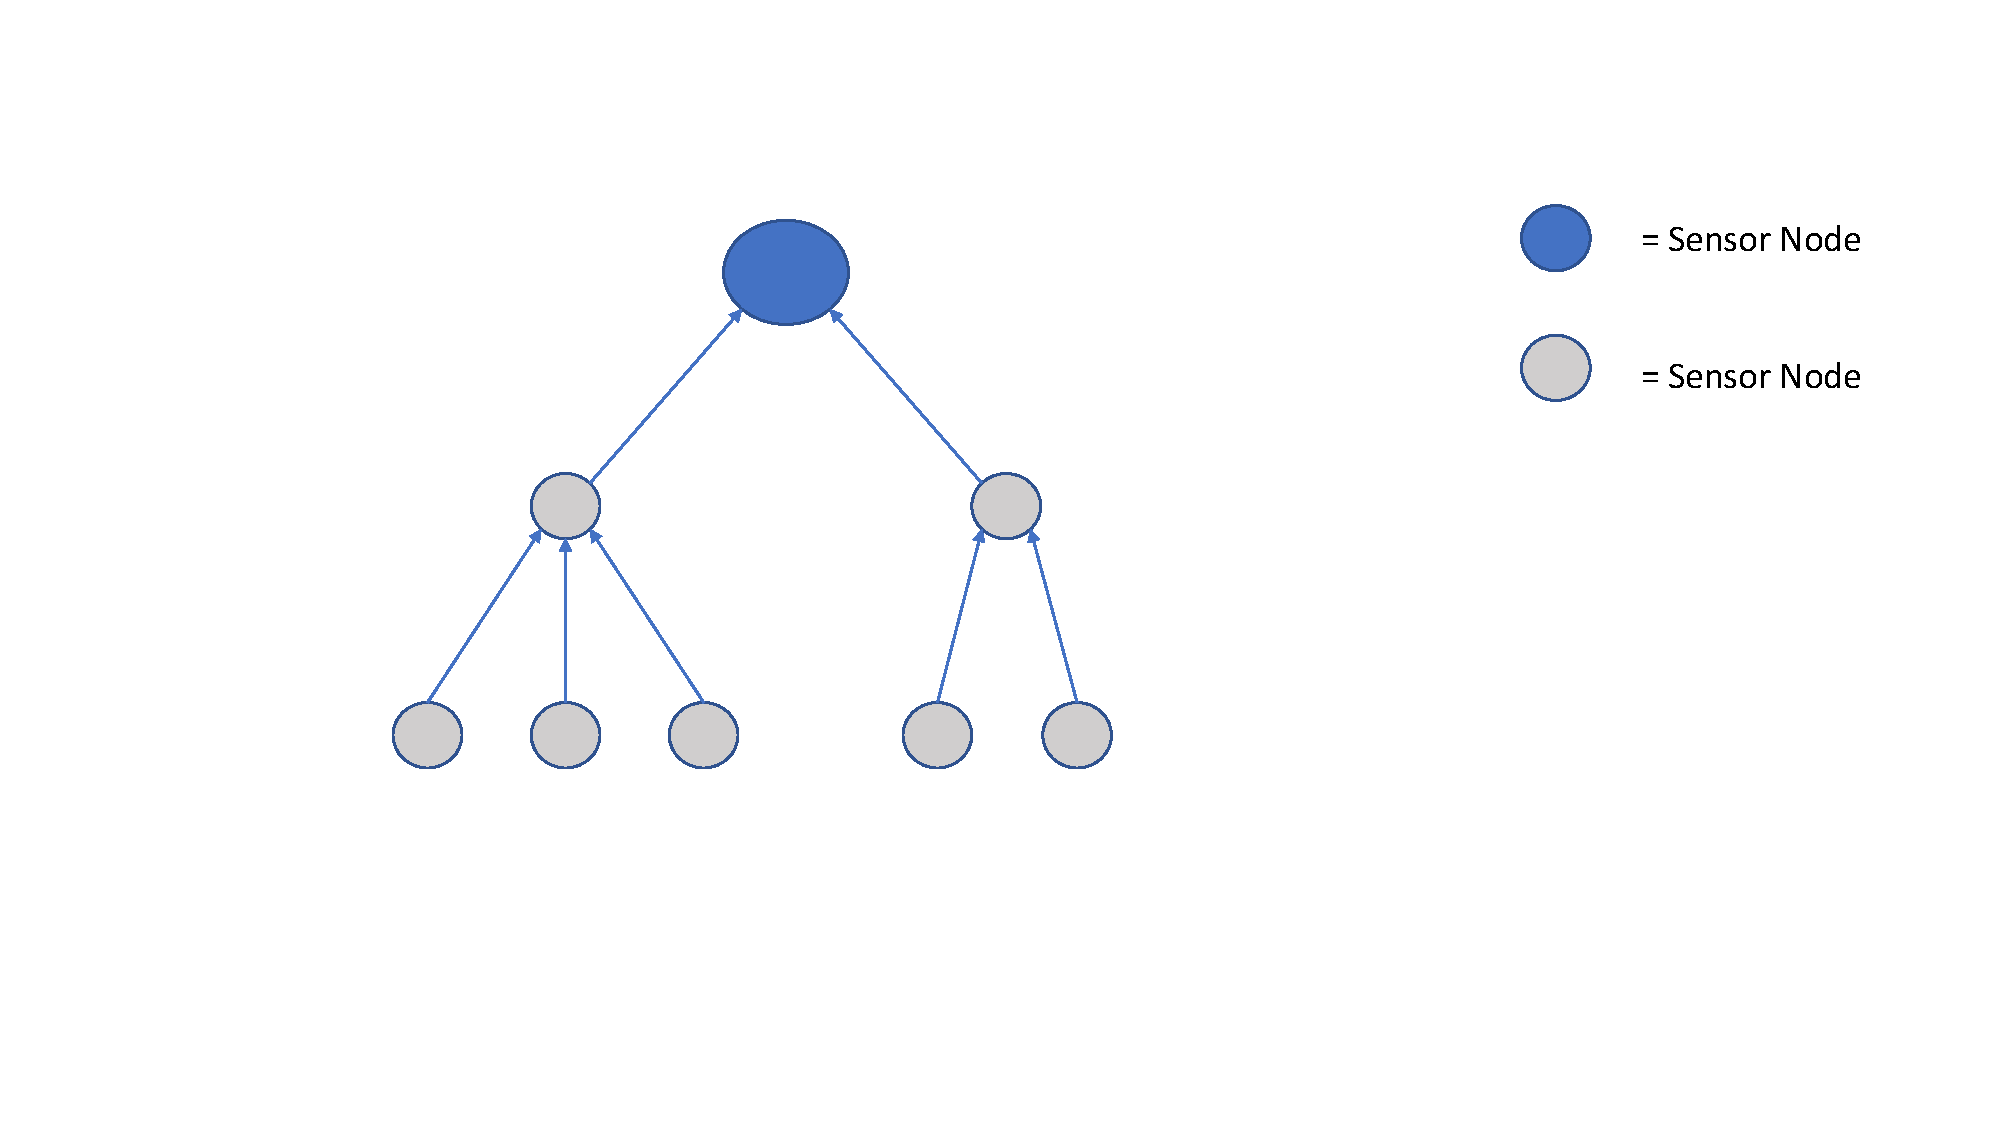
\includegraphics[width=\linewidth]{images/tree-structure.pdf}
%   \captionof{figure}{(a)}
%   \label{fig:Tree Topology}
% \end{minipage}
% \caption{Example Topologies. Inspiration taken from Reina et al.~\cite{reina2013role}}
% \end{figure}

\begin{figure}
\begin{subfigure}{.5\textwidth}
  \centering
  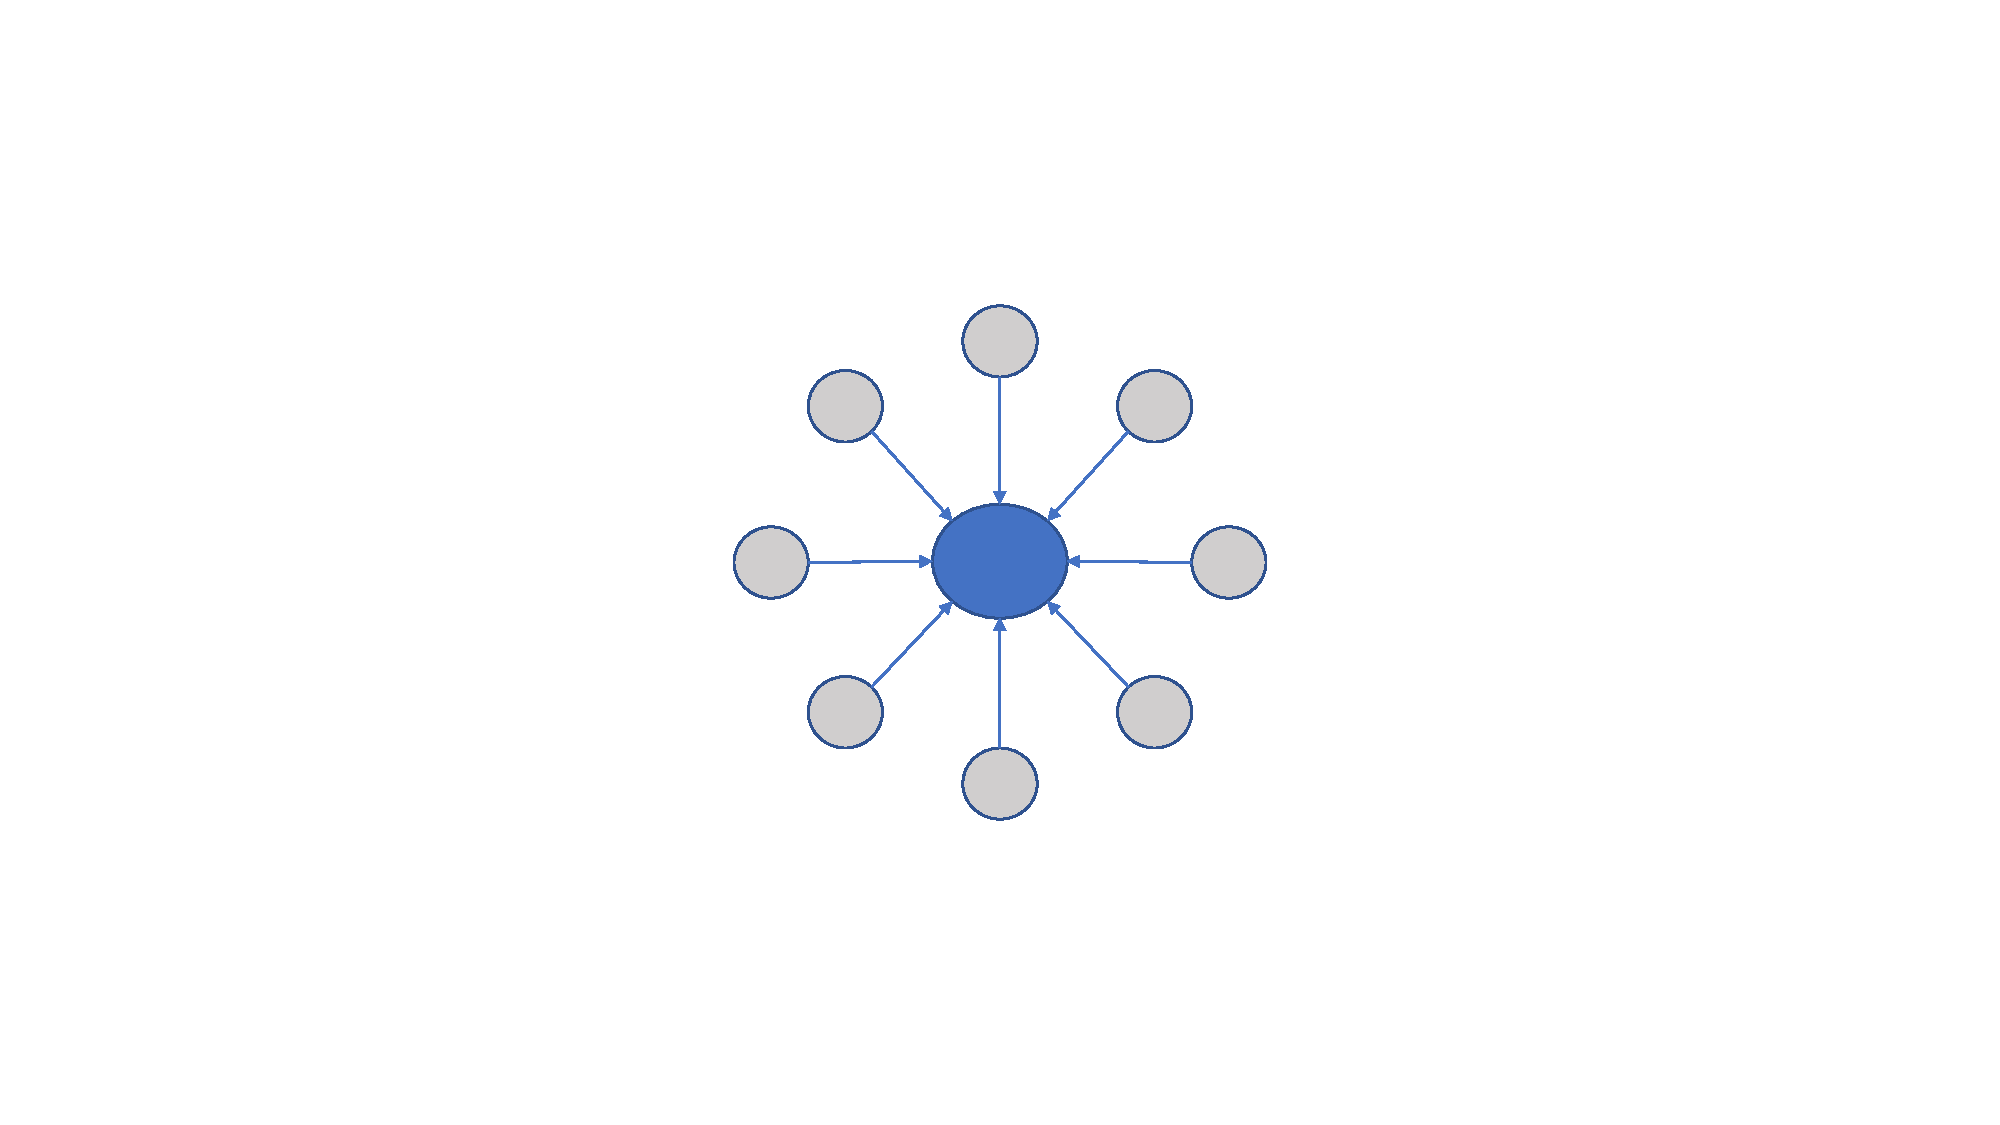
\includegraphics[width=.8\linewidth]{images/star-structure.pdf}
  \caption{}
  \label{fig:Star Topology}
\end{subfigure}%
\begin{subfigure}{.5\textwidth}
  \centering
  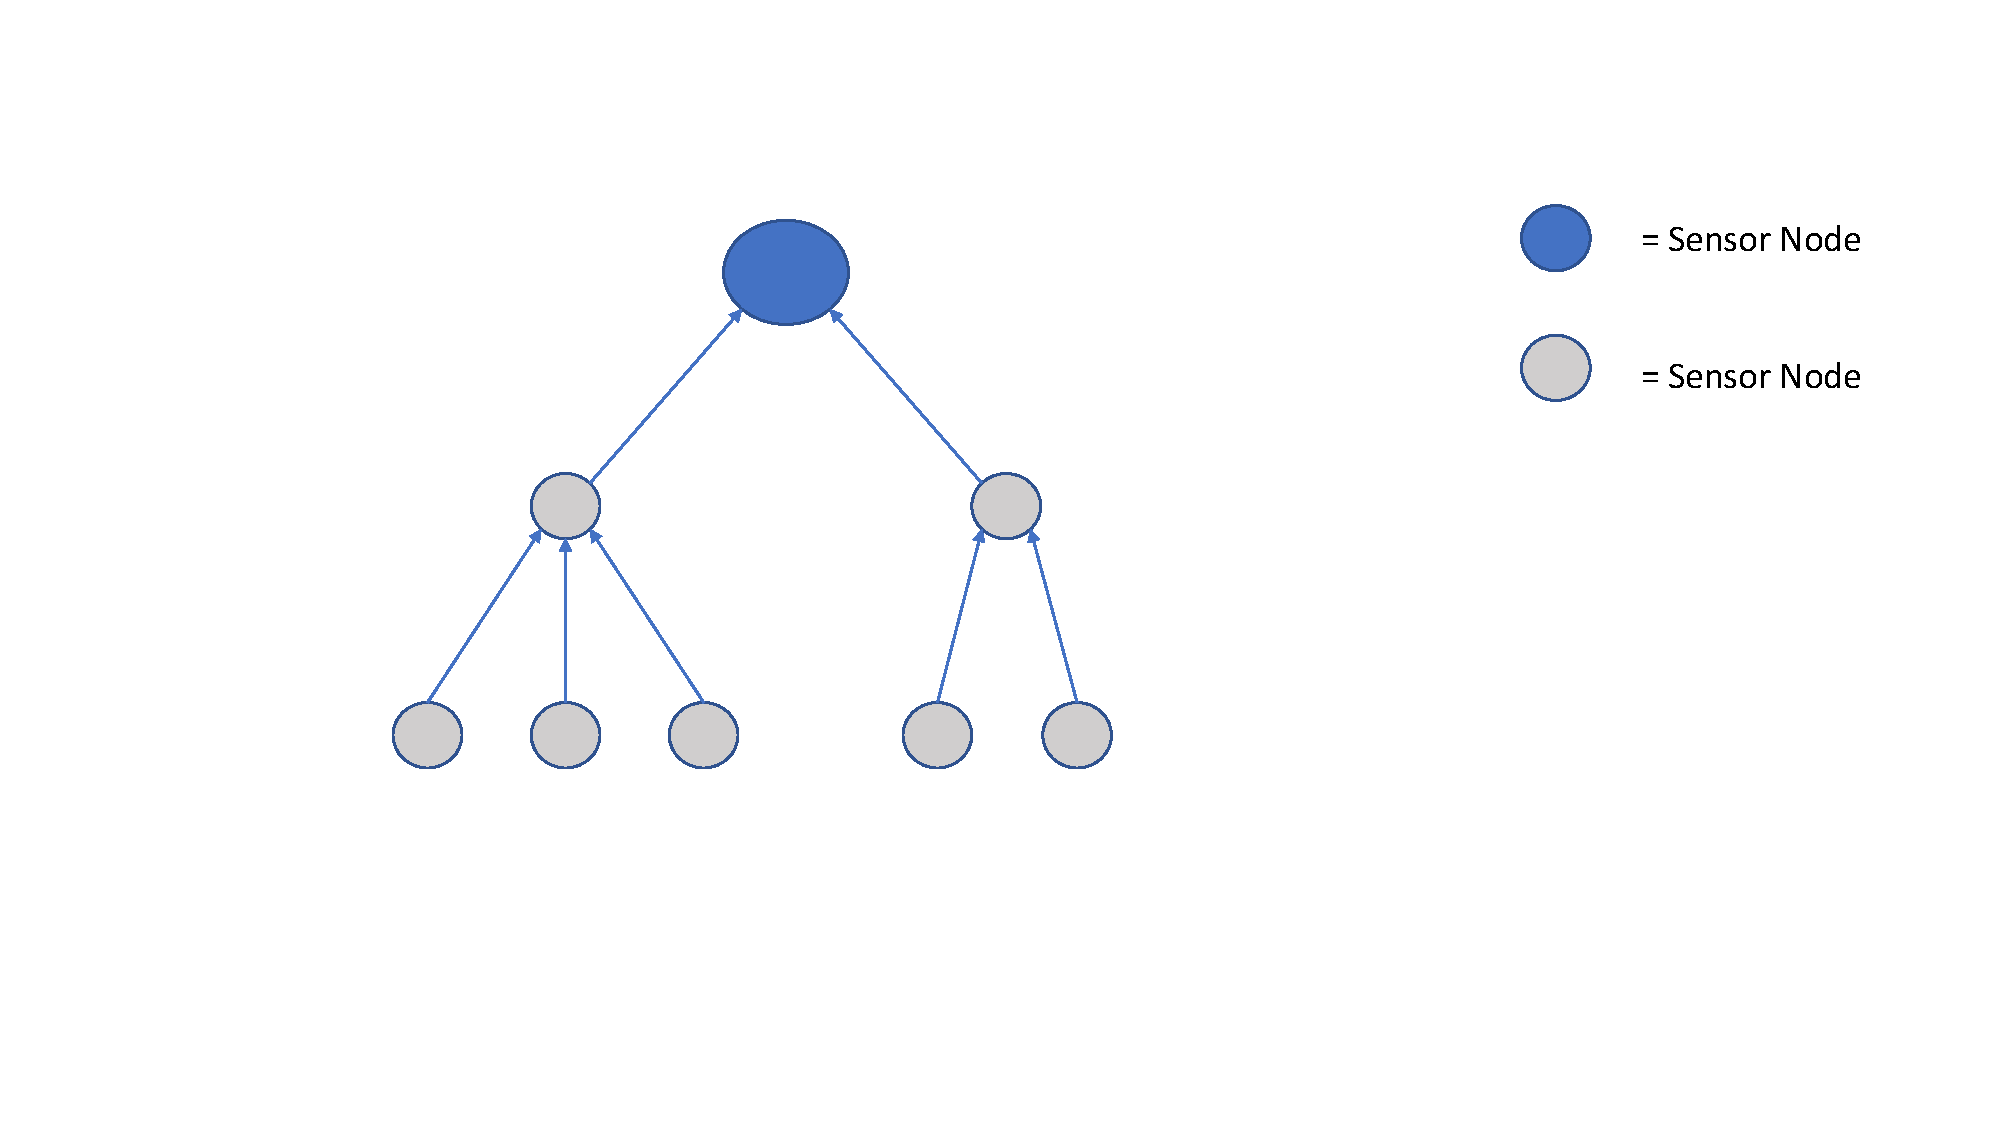
\includegraphics[width=.8\linewidth]{images/tree-structure.pdf}
  \caption{}
  \label{fig:Tree Topology}
\end{subfigure}
\caption{Example Topologies. Inspiration taken from Reina et al.~\cite{reina2013role}}
\label{fig:fig}
\end{figure}

\FloatBarrier


\subsection{Contributions}
\label{sec:contributions}

The contributions of this thesis go as follows: 
\begin{enumerate}
    \item We present a catalog of different sampling algorithms for sensor data
    gathering. We classify the sampling techniques in a taxonomy for a compact
    overview of the field of data sensing in \acp{SN}.
    \item We present relevant information for each algorithm. We define
    relevant information as:

        \begin{itemize}
            \item The problem(s) the algorithm tries to solve
            \item Basic workings of the algorithm
            \item Experimental results of the algorithm and how it compares to others
            \item Use case(s)
            \item Advantages and limitations of the algorithm
            % \item Compatibility of the algorithms with other techniques
        \end{itemize}

    \item We provide the basis for further research by presenting combinations
    of different algorithms.
    % TODO Add quantifiable point, e.g. number of algorithms presented and what we derived from it
\end{enumerate}


\subsection{Thesis Outline}

\para {Section \ref{sec:Methodology}.}  In section \ref{sec:Methodology}, we
explain our approach in compiling the taxonomy. In the first subsection we
define and discuss the terminology used in this work. The second subsection
motivates our selection criteria for including algorithms in the taxonomy. In
the third subsection we define out evaluation metrics for the presented
algorithms.

\para{Section \ref{sec:Taxonomy}.}  In section \ref{sec:Taxonomy}, we present a
taxonomy for classifying sampling algorithms. The section is split into four
subsections. The first gives an overview of the described classes and
subclasses and motivations for the classification. Each following section
describes a class and its subclasses in detail. For each subclass, relevant
information of multiple algorithms will be presented. 

\para{Section \ref{sec:Related Algorithms}.} In section \ref{sec:Related
Algorithms}, we review algorithms not covered in the taxonomy from areas other
than sampling, e.g. topology control and routing. This section is split into
two subsections. The first subsection presents those algorithms and their
relevant information. The definiton of relevant information for those
algorithms does not change. In the second section we discuss possible
combinations of different sampling algorithms with other sampling and
non-sampling algorithms. The combinations found here could be used as a basis
for further research.

\section{Methodology}
\label{sec:Methodology}

In this section we present our methodology in conducting our research. This
includes the selection criteria for including algorithms and publications into
the taxonomy and the evaluation metrics for the presented algorithms. We also
include a terminology subsection, where we discuss and define different terms
used in the area of data sampling and \acp{SN}.

\subsection{Terminology}
\label{sec:Terminology}

% TODO add a shit ton of definitions for every technical word used in the thesis

The literature related to data sampling from sensors defines many different
terms such as data collection (e.g.~\cite{laiymani2013adaptive, liu2007energy,
wang2012adaptive}), data sampling (e.g.~\cite{willett2004backcasting,
jain2004adaptive, szczytowski2010asample}), data gathering
(e.g.~\cite{wang2012data, luo2009compressive, zhang2016data}), and data sensing
(e.g.~\cite{padhy2006utility, mahmudimanesh2012balanced, duarte2005joint}).
Some publications use these terms as synonyms while other publications use
different terms to differentiate concepts. In the following paragraphs, we,
i.a. clarify the definitions of data collection, data sampling, data gathering,
and data sensing. We include this subsection, because we need to clarify the
terminology in order to be precise in the following sections. We will define
other terms used in this paper, aswell.

\begin{description}

    \item[Data Stream]
        Hirzel et al.~\cite{hirzel2014catalog} define data streams as "a
        conceptually infinite sequence of data items". We follow that
        definition in this thesis.
% TODO find better formulation than "follow that definiton"
    \item[Network Utilization]
        The standards for technology in automotive retail organization define
        network utilization as "the amount of traffic on the network compared
        to the peak amount that the network can support"~\cite{networkutil}. We
        follow that definition in this thesis.

    \item[Sampling Rate, Sampling Frequency]
        The federal agencies digital guidelines initiative defines sampling
        rate or sampling frequency as "the number of samples per second (or per
        other unit) taken from a continuous signal to make a discrete or
        digital signal"~\cite{samplingrate}. We follow that definition in this
        thesis.

    \item[Sensing Rate]
        

    \item[Sensor Node]
        

    \item[Base Station, Client Station, Fusion Center]
        


    \item[\ac{MAC}]
        

    \item[Duty Cycle, Duty Cycling]
        Lin et al.~\cite{lin2004medium} define a duty cycle as "the ratio of
        the listen interval to the frame length". Duty cycling is defined by
        Buettner et al.~\cite{buettner2006x} as an approach in which "each
        sensor node periodically cycles between an awake state and a sleep
        state".

% a frame length is the length of a data unit on the data link layer. A frame
% consists of a mac header and a payload (data)

    \item[Data collection and data gathering] 
        Data collection is often mentioned in connection with the whole process
        of acquiring data through sensors in \acp{SN}. A data stream produced
        by a sensor sensing a phenomenon is sampled by an sampling algorithm.
        The data is then routed through the network to the destination. The
        work of Yao et al.~\cite{yao2015edal} contributes, i.a., a technique,
        for finding the lowest cost path for sent data packages in a \acp{WSN}
        while additionally employing compressive sampling. The authors use data
        collection to define this process. Additionally, a survey by Di
        Francesco et al.~\cite{di2011data} defines the term data collection as
        the process of getting data from a sensor node to the sink node.
        Vukobratovic et al.~\cite{vukobratovic2010rateless} describe data
        gathering as the process of collecting sensed data from sensor nodes at
        specific sink nodes. A sink node could be a base station, e.g. a wired
        server, or another node in the \ac{SN} which acts as a gateway into the
        network and can route data to a server. We will use data gathering and
        data collection as synonyms as they both describe the whole process of
        acquiring data at sensor nodes and routing them to a base station.

    \item[Data sensing and data sampling] 
        The definitons for data sampling and data sensing are also inconsistent
        in the literature. Zhao et al.~\cite{zhao2016cats} employ sampling in
        the context of sink nodes assigning sampling tasks, which consist of a
        time window and a sampling interval, to sensor nodes. Trihinas et
        al.~\cite{trihinas2015adam} also do not differentiate between sampling
        and sensing.  Aquino et al.~\cite{aquino2014musa} on the other hand,
        discern sensing as the process of a preconfigured sensor unit measuring
        a physical phenomenon and sampling as the software taking samples form
        the data generated by the sensor unit. The distinction is important as
        the authors point out, that generally, an online reconfiguration of the
        sensor sensing times is not possible. Contrary, software is more
        flexible and sampling rates and intervals can be specified online.
        However, Deshpande et al.~\cite{deshpande2004model} argue, that a
        sensor can only provide \textit{samples} of an observed, continuous
        phenomenon. Therefore, additional sampling by an algorithm would be
        interpreted as filtering. To stay consistent with our differentiation
        between sampling and filtering, we will not distinguish sampling and
        sensing unless a presented work makes the distinction, e.g. an
        off-the-shelf sensor unit has a fixed sensing rate and can only be
        turned on or off. In such cases, the sampling is done on the data
        stream. Because sensor nodes have only limited
        memory~\cite{akyildiz2002wireless}, only \textit{samples} of the data
        stream would be stored at each point in time, on which additional
        filtering would be applied. This differs from reservoir sampling, ...
\end{description}
\par

\subsection{Algortihm selection criteria}
\label{sec:Algortihm selection criteria}


\subsection{Evaluation Metrics}
\label{sec:Evaluation Metrics}

\section{Taxonomy}
\label{sec:Taxonomy}

In this section we present our taxonomy of sampling algorithms for \acp{SN}. We
classify algorithms into two categories: \catI (Section~\ref{sec:catI}) and
\catII (Section~\ref{sec:catII}). %  and \catIII (Section~\ref{sec:catIII}).
\catI are all algorithms which prevent the \textit{sampling} of redundant data.
This is achieved at sensor node level, manipulating the sampling rate to
capture all relevant information from a data stream produced by a sensor. In
contrast, \catII focus on suppressing already sampled data by utilizing spatial
and temporal correlations between sampled values. We decided to include \catII
into the taxonomy, as filtering and sampling both take place at the sensor node
level and are applied before data is sent to data consumers.

% TODO Think about other points.

% IDEA: Talk about other ways, the algorithms could be classified. E.g.: Use
% case -> Tata et al. talk about how sensor network applications can be used
% for interval monitoring, i.e. report temperature in a room every hour or
% event monitoring, i.e. a bird lands in a nest, cars are counted in a traffic
% jam when one occurs, etc.

\subsection{Overview}
\label{sec:Overview}
% Picture of taxonomy at the beginning Explain picture and explain the terms
% e.g. model based adaptive sampling is a prediction scheme ... Reasoning
% behind the partitioning of the algorithms maybe if a assignment of a
% particular algorithm is not straightforward
% explain why thesis title is about sampling algorithms and taxonomy has 
% filtering and sampling as different categories

% Distinguish sampling algorithms, filtering algorithms and data sharing from
% each other

\subsection{\catI} % Sampling Algorithms
\label{sec:catI}

The first category of our taxonomy incorporates all algorithms which primary
focus is on manipulating the sampling or sensing rate of one or multiple sensor
nodes to reduce network utilization. Although there are algorithms from other
categories which also may incorporate manipulations to the sensing/sampling
rates of sensor nodes (e.g.~\cite{trihinas2015adam, jain2004adaptive}), we
include algorithms to the Sampling Algorithms category only if the main focus
of the work lies on sampling rate manipulation. % maybe rewrite that

In our research we found adaptive sampling and compressive sampling to be good
sub classifications for sampling algorithms. Both types of algorithms target
sampling rates of sensor nodes to reduce network traffic. Adaptive sampling
algorithms employ schemes to dynamically react to changes in the behaviour of
an observed phenomenon, by manipulating sensing rates of sensor nodes.
Compressive sampling utilizes findings from the field of signal processing, to
sample signals, i.e. data streams from an observed phenomenon, below the
typical Nyquist rate~\cite{candes2008introduction}. From such a subset of data,
the original signal can be reconstructed at sink node or base station with very
high accuracy.

\subsubsection{Adaptive Sampling}
\label{sec:Adaptive Sampling}

% All required definitions for adaptive sampling
Trihinas et al.~\cite{trihinas2015adam} define adaptive sampling as:

\begin{quote}
    "The process of dynamically adjusting the sampling rate to the current
    metric evolution, such that when stable phases in a metric stream are
    detected, the sampling rate is reduced to ease processing and energy
    consumption."
\end{quote}

\par
Although the quote is from 2015, the idea of adaptive sampling goes back to the
2000s. One technique called \textit{Backcasting} was presented by Willet et
al.~\cite{willett2004backcasting}. The key idea of the work is that a monitored
environment exhibits correlations in time and space domains which can be
exploited to reduce the number of required sensor nodes to deliver an accurate
picture about the monitored environment. The authors assume that the sensor
network is a rectangular field of uniformly distributed sensor nodes.
Initially, a subset of the sensor nodes is chosen by the fusion center to
provide an initial estimate of the sensed phenomenon by a recursive dyadic
partition. A subset of nodes are mutliple clusters of nodes with a cluster head
each. Cluster heads route the data from the sensor nodes to the fusion center
and vice versa. The fusion center recieves the sensed data and activates
additional nodes to improve the quality of the sampling by reducing the
\ac{MSE}. The authors evaluate their approach theoretically and come to the
conlusion, that a \ac{WSN} with 10000 sensors and energy to operate
continuously for a year, would operate for 10 years when using
\textit{Backcasting}. The authors point out that network lifetime could be
improved if mechanisms for cycling the position of cluster head would be
implemented. Altough the algorithm does not manipulate the sampling rates of
individual sensor nodes it is still one of the first algorithms to adaptively
change the sensing tasks of nodes based on the dynamics of the observed
phenomenon.

\par

Another technique, also from 2004, was published by Jain et
al.~\cite{jain2004adaptive}. The authors main contribution is an algorithm to
change the sampling rate of individual sensor nodes in a stream sensor network
based on the importance of the observed data. An important event could be a
camera observing non-standard driving behaviour of a car, e.g. driving in a
zigzag course or a temperature spike in a data center. At sensor node level,
kalman filters predict sensed values. They are then compared against the actual
sensed values. The values are stored in a sliding window locally. An estimation
error is computed over the sliding window. The estimation error indicates a
changing dynamic of a observed phenomenon. After each taken sample, a sensor
node adjusts its \ac{SI} i.e. the time interval between two consecutive
samples. If the desired \ac{SI} lies in the \ac{SIR}, the sensor node can
adjust its \ac{SI} locally. Otherwise the sensor node has to request a new
\ac{SI} from the server. The server keeps a metric of avaliable communication
resources which gets updated after a request to change a \ac{SI} is accepted.
The requests are stored in a job queue. To approve a \ac{SI} a linear
optimization problem has to be solved. The authors evaluated their approach on
synthetic data generated by a spatio-temporal data generator. Tested metrics
where the mean fractional estimation error $ \eta $, the proportion of messages
exchanged between the source and the server and the number of values sensed by
the source nodes \textit{m}. The adaptive sampling algorithm outperformed the
alternative uniform sampling algorithm almost in every test. Tests were done,
i.a using different numbers of sensor nodes and sliding window sizes. The
authors indicate, that the algorithm is not applicabble to multi-hop sensor
networks, i.e. a sensor node has to have a direct connection to the server.
Furthermore, both the sliding window and the \ac{SIR} have to be chosen by the
user. Also, the authors state that the message overhead is high. The main goal
of the algorithm is to optimize bandwidth usage in the network, thus this
technique is more suitable for wired \acp{SN} and less for \acp{WSN} as the
communication overhead is high and communication consumes a major amount of
energy in most sensor nodes~\cite{raghunathan2002energy}.

\par

A technique designed initially for a glacier monitoring application by Padhi et
al. \ac{USAC}~\cite{padhy2006utility} is an example of an adaptive sampling
scheme for a \ac{WSN}. The algorithm uses a linear regression model at each
sensor node to capture phase shifts of the observed phenomenon as fast as
possible. The model predicts values at a sensor node. Those values are checked
against the actual sensed values. If a predicted value lies in the user defined
\ac{CI}, then the sensor node reduces its sampling rate by a multiplicative
factor $ \alpha $ until the sampling rate reaches $ f_{min} $. $ f_{min} $ is
set by the user. If the value does not lie in the \ac{CI} then the sensor node
raises its sampling rate to $ f_{max} $ to capture a supposed change in the
dynamic of the observed phenomenon. The experiments tested the algorithm
against the older deployed protocoll in the glacier monitoring application
\textit{GLACSWEB}. In the \textit{GLACSWEB} protocol, sensor nodes send their
data directly to the sink node. This technique is energy unefficient as the
authors state that 

\begin{quotation}
    "(...) the power required to transmit data from one
    node to another is proportional to the square of the distance
    between the nodes (...)."
\end{quotation}

Additionally, \textit{GLACSWEB} has a static sensing rate which the authors
argue, induces unnecessary sampling.

The tests were conducted in a simulated environment using
historical data from the application. The authors tested different network
topologies, numbers of sensor nodes in a network and number of changes in the
dynamic of the data. The experiments resulted in \ac{USAC} outperforming the
older algorithm in every test. The efficiency increase, which is defined by the
authors as

\begin{quotation}
    "The value of the data gained over the energy consumed of USAC relative to
    GLACSWEB in each case."
\end{quotation}


was, i.a. 470\% when distributing sensor nodes randomly around a center base
station.
\par

\acp{RSN} combine the perpetual operation lifetime of wired \acp{SN} and the
flexibility of \acp{WSN}. However, \acp{RSN} introduce new challanges for
designing data collection algorithms. A paper from Srbinovski et
al.~\cite{srbinovski2016energy} presents an adaptive sampling algorithm for
\acp{RSN} with energy hungry sensors. The authors point out, that contrary to a
common assumption that communication consumes most of the energy in sensor
nodes (e.g.~\cite{santini2006adaptive}), the sensor unit can be the main energy
consumer~\cite{boyle2012energy}. The authors contribute an \ac{EASA} for
perpetually operating \acp{RSN} which builds upon the \ac{ASA} by Alippi et
al.~\cite{alippi2007adaptive}. The \ac{ASA} algorithm leverages the Nyquist
Theorem $$ F_N > 2 \cdot F_{max} $$ for finding the optimal (minimum) sampling rate
$ F_N $. To estimate the maximum frequency in the power spectrum $ F_{max} $, a
\ac{FFT} is used on the first $ W $ samples of the process. A \ac{CI} can be
defined to capture changes in the dynamic of the process. The algorithm is run
on the base station due to computational complexity, thus some communication
overhead is present. \ac{EASA} expands \ac{ASA} with energy awareness, i.e.
adjusting optimal sampling frequency of a sensor node based on current and
critical battery level, and rate of energy saving. When the battery level drops
below the user defined critical value $ m $, the sampling rate deviates from the
optimal \ac{ASA} sampling rate. This may lead to the signal not capturing the
singal fully as the nyquist theorem is violated. The authors argue that a
potential loss in data quality is the cost of staying continuously in the
network. The authors tested \ac{EASA} extensively on data from two deployments.

\begin{enumerate}
    \item A custom, windpowered deployment for measuring wind speed
    \item An off-the-shelf solar powered deployment for measuring $ CO_2 $ in a beehive
\end{enumerate}

\ac{EASA} was tested with different saving rates against \ac{ASA} and
addtionally on the second deployment against a fixed rate. All tests were done
in a simulated environment. In both delployments, \ac{ASA} and \ac{EASA} have
the same sampling rate when the battery level is above $ m $. \ac{ASA} can
deliver a high data quality, as the sampling rate is always optimal. \ac{EASA}
on the other hand, stablelizes in the first deployment the energy levels of the
sensor node after 36 days of operation at $ 60\% $ with an $ m $ of $ 1/3 $.
With \acp{ASA} the energy levels are at $ 20\% $. In the second deployment,
\ac{ASA} gets outperformed slightly in energy consumption by \ac{EASA}. The
energy levels with the fixed sampling rate are depleted after 13 days.

% Adaptive Monitoring by Tata and MEGAhed. Goal: Determine metrics which should
% be monitored and the frequencies with which they should be monitored. 


\subsubsection{Compressive Sampling}
\label{sec:Compressive Sampling}

\ac{CS} is a relative new sampling paradigm which was first
introduced by Donoho et al.~\cite{Donoho06compressedsensing} in 2006. 
Mahmudimanesh et al.~\cite{mahmudimanesh2010reordering} describe \ac{CS} as:

\begin{quotation}
    \ac{CS} states that it is possible to reconstruct a discrete signal from a set of
    randomly chosen values selected from a vector computed by a linear transform
    of the discrete signal vector.
\end{quotation}

Candés et al.~\cite{candes2008introduction} summarize the main principles of
\ac{CS} as sparsity and incoherence. A signal is sparse when "[it] contains
only a small number of non-zero elements compared to its
dimension"~\cite{elzanati2015collaborative}. Candés et al. define incoherence
as when a sample of a sparse signal has an "extremely dense" represention in
some domain $ \Psi $~\cite{candes2008introduction}. Luo et
al.~\cite{luo2009compressive} give an example of a signal being sparse in
\ac{DCT} domain in Fig.~\ref{fig:sparsesignal}.

\begin{figure}
\centering
\begin{minipage}{.5\textwidth}
  \centering
  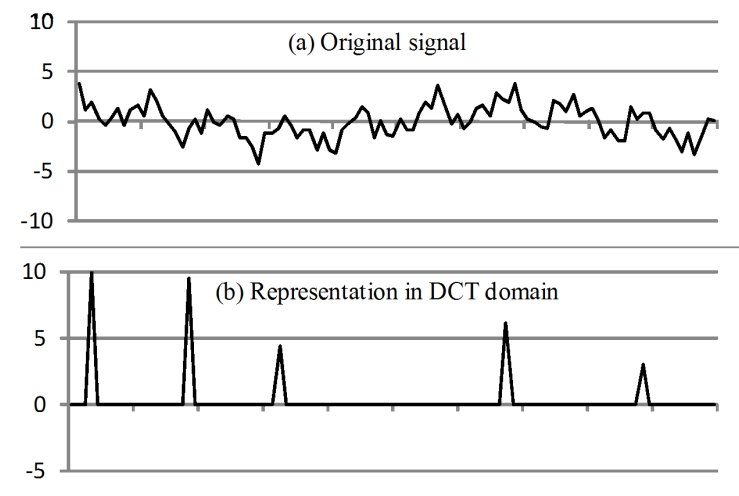
\includegraphics[width=\linewidth]{images/example-signal-sparse.png}
  \captionof{figure}{A sparse signal in the DCT domain~\cite{luo2009compressive}}
  \label{fig:sparsesignal}
\end{minipage}%
\begin{minipage}{.5\textwidth}
  \centering
  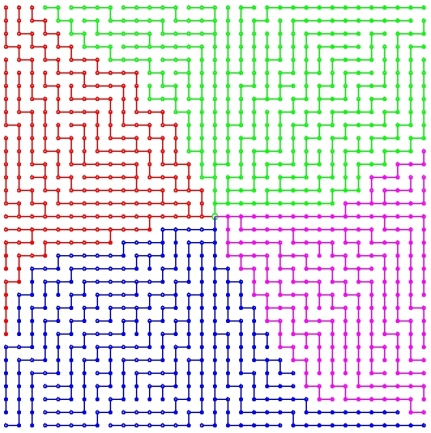
\includegraphics[width=\linewidth, height=5.2cm]{images/grid-topology-luo.png}
  \captionof{figure}{A grid topology~\cite{luo2009compressive}}
  \label{fig:grid topology}
\end{minipage}
\end{figure}

% CDG
% make a different introduction if you dont find a paper which could intrduce cdg
Compressive sampling methods were designed for large scale, multihop sensor
networks, aswell. Luo et al.~\cite{luo2009compressive} developed a \ac{CDG}
algorithm for large scale sensor networks. The goal of the algorithm is to
deacrease energy expenditure and distribute energy consumption evenly across
all sensor nodes to maximize the lifetime of the network. This is achieved by
reducing the datatraffic in a network by compressing data readings at each hop.
This would lead to $ M $ messages arriving at the sink from $ N $ sensor nodes,
where $ M << N $. The sink broadcasts a random seed to the network with which
each sensor node can generate, together with its own identificator, a local
seed. Sensor nodes then use the local seed to generate a random coefficient $
\phi_i $ which they transmit together with their sensor reading $ d_i $ to
their parent node. Parent nodes receive readings from their child nodes and sum
the input with their own $ d $ and $ \phi $. Therefore, every sensor node
transmits only one value. This ensures the sink node receives $ M $ weighted
sums $ y $, which consist of a matrix of the random coefficients, $ \Phi $ and
all sensor readings \textbf{d}:

$$
\begin{pmatrix}
    y_1 \\
    y_2 \\
    \vdots \\
    y_M
\end{pmatrix}
=
\begin{pmatrix}
    \phi_{11} & \phi_{12} & \dotsb & \phi_{1N}\\
    \phi_{21} & \phi_{22} & \dotsb & \phi_{2N}\\
    \vdots & \vdots & \vdots & \vdots\\
    \phi_{M1} & \phi_{M2} & \dotsb & \phi_{MN}\\
\end{pmatrix}
=
\begin{pmatrix}
    d_1 \\
    d_2 \\
    \vdots \\
    d_N
\end{pmatrix}
$$

The random matrix $ \Phi $ is not transmitted because the sink can compute the
matrix if it knows the identificators of the sensor nodes. The original
sensor readings \textbf{d} can be reconstructed at the sink by solving:

$$
\displaystyle{\min_{x\in R^N} \ ||x||_{l_1}}  \ \ \   s.t.  \ \  y = \Phi \textbf{d} , \ \ 
\textbf{d}  = \Psi x
$$

$ \Psi $ is the domain in which \textbf{d} can be represented by $ K << N
$ coefficients and $ x $ is the vector of coefficients.

The authors evaluated \ac{CDG} against a baseline transmission scheme (all
nodes transmit as soon as readings are aquired) with the ns-2 simulation
tool~\cite{bajaj1999improving}. Additionally, testing was done on two real life
datasets to evalutate the reconstuction capability. For the simulated
environment, the authors created two synthetic sensor networks. The first is a
network with a chain topology, with 1000 sensor nodes spaced 10 meters apart
from each other and with sink nodes located at each extreme of the chain. The
second set-up was a grid-like routing tree with 1089 sensor nodes and a sink
node in the center of the network, e.g. Fig.~\ref{fig:grid topology}. The
authors varied in their testing runs the signal input intervals and observed
the package loss and output interval change. \ac{CDG} outperformed the baseline
scheme in both topologies managing input intervals 5 times and 2.3 times
smaller than the baseline scheme in the chain and grid topologies respectively.
Additionally, \ac{CDG} achieved a packet loss of near zero in both topologies,
while the baseline scheme had package loss rates of 5\% and 20\% in the chain
and grid topologies respectively.

The real life datasets consist of measurements collected in the Pacific Ocean
by a single moving device and a sensor network in a datacenter. The authors
argue that the Pacific Ocean dataset has the same properties as data collected
by a sensor network. The authors found the Pacific Ocean data to be sparse in
wavelet domain. \ac{CDG} can reconstruct the initial 1000 datapoints from 40
datapoints with $ > 98\% $ precision. The datapoints are the 40 highest
coefficients in the wavelet domain of the data. The authors did not find a
sparse representation of the datacenter dataset as the data exhibit little
spatial correlation. Instead they opted for reorganizing the dataset by sorting
the temperature values in ascending order at a moment $ t_0 $. The result is
sparse in the wavelet domain and the original signal can be reconstructed.

% \begin{figure}[h]
% 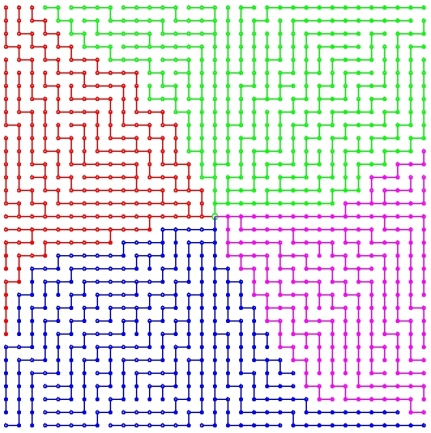
\includegraphics[width=8cm]{images/grid-topology-luo.png}
% \caption{A grid topology~\cite{luo2009compressive}}
% \label{fig:grid topology}
% \centering
% \end{figure}

\par

One paper by Cheng et al.~\cite{cheng2010efficient} builds upon the low rank
feature of a matrix. The authors point to discoveries proving that a matrix
formed from spatial and temporal correlated data is approximately low rank and
can be recovered from a subset of the data~\cite{vuran2004spatio,
candes2009exact}. With the \ac{EDCA} sensor nodes sample at a fixed rate and
send their sensed values to a cetral sink in a multi-hop scheme. However, the
authors point out that missing values, i.e. no values in some time slots, can
be recovered with low error. The focus of the algorithm lies on the recovery of
a low rank
% Therefore, the sampling rate could be made dynamic to further increase
% efficiency.
matrix. The authors use the nuclear norm to solve the rank minimization problem

$$
minimize \ rank(X), \ s.t. \ A(\cdot)=B
$$

where $ X $ is the matrix arriving at the sink and $ A(\cdot) $ is an operator
representing the incompleteness of the matrix. Because the problem is NP-hard,
the authors use a heuristic and shift the problem to a convex optimization
problem

$$
minimize \ || \ A(LR^T) - B \ ||^2_F + || \ L \ ||^2_F \ + || \ R \ ||^2_F
$$

where $ X $ is deconstructed with \ac{SVD} into $ X = U \Sigma V^T $ and $ L =
U\Sigma^{1/2}; \ R = V\Sigma^{1/2}$. The problem is solved using a method by
Zhang et al.~\cite{zhang2009spatio}.

Testing was done using a publicly availiable dataset of temperature
measurements by sensor nodes from the berekeley Research Laboratory and a
synthetic dataset. With the real world data, the authors tested the accuracy of
\ac{EDCA} while using different sampling ratios for the 54 sensor nodes. The
authors could only observe small recovery errors. With a sampling ratio of 0.2,
i.e. every fifth sensed value is transmitted, the standard deviation $ \sigma $
was $ < 0.15°C $. % Reread that, as in stcdg, edca does not perform that well
With the synthetic data set, the authors compared \ac{EDCA}
with a naive scheme, in which all sensed data points are sent to the sink, on
network lifetime. The lifetime of a sensor network is defined by the authors as
"the time duration of the first sensor node which runs out of power". The
lifetime ratio is defined as $ (1/M_{max}) / (1/M_0) $ where $ M_{max} $ is
"the maximum power wasted [...] on every simulation using \ac{EDCA} and $ M_0 $
the power wasted by the naive scheme. The authors found the lifetime ratio to
be 5 when having a sampling ratio of 0.2, increasing the lifetime of a network
fivefold in comparison to the naive scheme.


\par

% stcdg
Another paper by Cheng et al.~\cite{cheng2013stcdg} expands \ac{EDCA} and
introduces a \ac{STCDG} algorithm. Similiar to \ac{EDCA}, \ac{STCDG} exploits
the low rank feature and the short-term stability of data gathered through a
\ac{SN}. The authors argue, that, unlike \ac{CDG}, \ac{STCDG} is more flexible
and does not have to be customized for a specific \ac{SN}. This comes from the
fact, that with \ac{CDG}, the domain in which the data is sparse has to be
known in advance. Additionally \ac{CDG} utilizes only the sparsity of data,
requiring the full dataset to be reordered if the data is not sparse.

The authors deployed an own sensor network in a residential building. They used
the data to analyze short-term stability and low rank of spatially and
temporally correlated data. The authors found the data to have a good low-rank
approximation and short-term stability. Short-term stability is defined by the
authors as the difference between adjacent gaps of sensor readings, with gaps
being the time between two adjacent sensor readings. So the difference is
defined as 

$$
dif(n,t) = X(n,t + 1) + X(n,t - 1) - 2X(n, t); \ \ where  \ \ 1 <= n <= N  \ \ and  \ \ 2 <= t <= T - 1
$$

thus, if $ dif(n, t) $ is small then sensor readings at node n around timeslot
t are stable.

The authors expanded their optimization problem formulation to include a tuning
parameter $ \zeta $ to tradeoff fitting the algorithm to the data and achieving
low rank. With the short term stability added into the optimization problem, as
the difference for all data points in the original matrix $ X $, $
||(LR^T)S^T||^2_F $ the optimization problem is now

$$
minimize \ ||(LR^T). \cdot Q-B||^2_F + \zeta(||L||^2_F + ||R||^2_F) + \eta ||(LR^T)S^T||^2_F
$$

Another extentsion of \ac{STCDG} is the handling of empty columns. Empty
columns may appear at the sink when the sampling ratio is low or the packet
loss rate is high. The authors point out that such cases can lead to very high
recovery errors. Therefore, the algorithm ignores empty columns first and
recovers the original matrix. The empty columns are seperately filled using the
short-term stability feature. Additionally, abnormal values sensed by sensor
nodes are transmitted independant of the set sampling ratio.

The authors tested \ac{STCDG} against \ac{EDCA} and \ac{CDG} on 3 different
datasets in terms of recovery error, power consumption and network capacity.
The used datasets were the berekeley Research Laboratory sensor data, a
synthetic trace generated with the ns-2 tool~\cite{bajaj1999improving}, and the
residential building data gathered by the authors. Specifically, the authors
subdivided the laboratory and residential building data sets into singular
sensed phenomena, namely light and temperature. \ac{NMAE} was used to measure
the recovery performance of the algorithms. The researchers found that the
algorithms have critical sampling ratios, which if surpassed, lead to a high
\ac{NMAE}. \ac{STCDG} perfomed better than the other algorithms, having low
\ac{NMAE} (sub 0.1) with low sampling ratios (0.1 - 0.2). \ac{CDG} perfomed
worst of all. The authors argue that the sparsity feature is not always present
in real life data sets. The performance of all algorithms dropped on datasets
with lower temporal/spatial correlation and fewer sensor nodes (24 and 54
sensor nodes in the residential building and laboratory datasets respectively).
The authors argue that \ac{CDG} is outperformed at high sampling ratios by a
centralized exact scheme, which, like the naive scheme in the previous work of
Cheng et al.~\cite{cheng2013stcdg}, sends all sensor readings at every timeslot
to the sink. \ac{STCDG} and \ac{EDCA} have both the same energy consumption.


\subsection{\catII} % Filtering algorithms
\label{sec:catII}

The second category of our taxonomy contains algorithms which primary focus
lies in reducing data sent through the network after it is sampled. The
subclassifications deal with adaptive filtering and prediction based schemes.
Prediction based schemes focus on using probabilistic models to suppress sensor
readings if the readings can be predicted with acceptable accuracy at another
sensor node or sink. The algorithms presented include additional schemes, e.g.
clustering, to further reduce communication between nodes without reducing
prediction accuracy under some threshold. Adaptive filtering algorithms include
techniques to suppress sensed values based on temporal and spatial correlations
in the network.

% here adaptive filtering summary
% introduction or outlook to that category after writing the subsubsection parts

\subsubsection{Model Based Schemes}
\label{sec:Model Based Schemes}

We categorize algorithms into model based schemes if they use a prediction
model to enrich delivered sensor data at a sink or replace data transmission
altogether. One of the earlier examples of a model driven data gathering
technique is the well cited work of Deshpande et al.\cite{deshpande2004model}.
The authors present \textit{BBQ} (or Barbie-Q) a model query system in which
user's queries to a sensor network are answered, until some error threshold,
with a prediction model. Only if the prediction is not accurate enough, actual
sensed values are transmitted through the network. \textit{BBQ} is a query
processing engine, capable to process user queries similiar to \ac{SQL}. The
researchers make a general point in favour of model based schemes to answer
user queries. The authors argue that besides easing the communication load on
the network, statistical models can also, i.a. identify faulty sensors and fill
holes the network by extrapolating missing data. The authors use a timevarying
multivariate Guassian model, however they point put that their framework is
model agnostic. In \textit{BBQ}, a model is constructed (or trained) using
historical data, therefore some initial sensed values need to be collected in
order to initialize the model. Afterwards, users can query the network, e.g.
ask for the temperature sensed by a group of sensors with an error margin and a
confidence interval. \textit{BBQ} then tries to answer the query, minimzing the
amount of sensor nodes asked. Based on the underlying model, the system builds
an observation plan which specifies how and in which order sensor nodes are
queried. The "how" refers to the model choosing another attribute to query
instead. The reason behind this is that some attributes, like temperature and
voltage, are highly correlated. The authors show, that the correlation can be
leveraged by the model, as voltage is sometimes cheaper to sample than
temperature. Additionally, spatial and temporal correlations are leveraged by
the model to reduce the number of sensors queried.

The authors evaluated their system by comparing \textit{BBQ} with
TinyDB~\cite{madden2005tinydb} and Approximate-Caching on two datasets
collected by a small amount of sensors (11 and 54 each). TinyDB is a sensornet
querying system in which the readings of sensor nodes are send and aggregated
on the way to the sink. With Approximate-Caching, sensor nodes send their
sensed values to a sink only if they differ from the previous sent values by
some user defined margin $ \epsilon $. So in comparison, TinyDB reports always
the exact values asked for in a user query, while  Approximate-Caching is
tweakable with error bounds and \textit{BBQ} is additionally configurable with
\acp{CI}. Therefore, the acquisition costs of TinyDB were constant while
\textit{BBQ} outperformed the other algorithms on high error margins ($
\epsilon = 1 $) with acquisition costs being an order-of-magnitude lower than
those of Approximate-Caching. As the authors themeselves point out,
\textit{BBQ} is not suitable for anomaly detection, as for such a task constant
sensor sampling is required.
\par
Chu et al. tackle, i.a., this problem, in their work~\cite{chu2006approximate}.
The presented algorithm, \textit{Ken} targets \textit{SELECT *} queries in
which all values are requested from all sensor nodes. No data reduction takes
place and such queries are thus expensive regarding energy consumption through
communication. \textit{Ken} operates using a prediction model which is
synchronized at the sink and at sensor nodes. Users query the sensor network
with frequency and error interval arguments, e.g. values from all sensor nodes
every f seconds with an error margin of $ \pm\epsilon $. A sensor node collects
values and checks if the sink node is able to predict the collected values
correctly within $ \pm\epsilon $. If the values lie within the interval, the
sensor node suppresses its reading. In the other case, the sensor node pushes
its values down the network to the sink node which in turn forwards the
readings to the base station. The models at the sink node use the new values to
\textit{resynchronize} its model with the model at the sensor nodes. In a
multihop \ac{SN}, additional compression based on spatial correlation can take
place at different hops. To enable compression based on spatial correlation,
the authors propose a clustering scheme in which there are multiple sink nodes
which communicate with the base station. This reduces communication overhead,
as sensor readings do not have to be stored in one central place in the
network. Each sink node maintains a synchronized prediciton model with its
child nodes. Additionally, the base station maintains synchronized prediciton
models with the sink nodes. Such a structure is depicted in
Fig.~\ref{fig:cluster Chu}. To find such clustering groups, the authors, i.a.,
present a heuristic approach, in which sensor nodes are assigned to a sink node
by its data reduction factor, i.e. a performance indicator for the prediciton
model. The authors evaluated their approach on two real world datasets with
small, fixed amount of sensors (one with 11 and the other with 49 sensors).
\textit{Ken} was tested with the clustering technique and with an average
model, in which predictions are made with the average of all sensed values and
no clusters are build. The authors came to the conclusion, that \textit{Ken}
performs better with the clustering scheme, when the communication costs to the
base station are many times higher than to a neighbor. This advantage recedes if
there are a lot of outliers which the model cannot predict.

\begin{figure}[h]
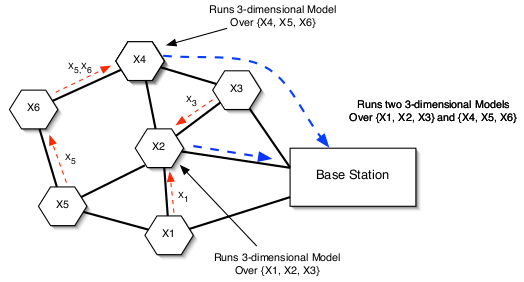
\includegraphics[width=\linewidth]{images/ken-clustering.png}
\caption{Example of a \ac{SN} with clusters by Chu et al.~\cite{chu2006approximate}}
\label{fig:cluster Chu}
\centering
\end{figure}

\par
Gedik et al. point out in their work, that \textit{Ken} is uneffective when the
observed phenomenon changes unpredictably over time~\cite{gedik2007asap}. In
such cases, the prediction model has to be adapted or reconstructed, which
introduces high communication overhead if the model is constructed centrally at
the base station. Additionally, the authors of \textit{Ken} did not take the
extra energy expenditure of clusterheads/sinknodes have, compared to regular
sensor nodes, into account. Gedik et al. address these issues in their
algorithm, \textit{ASAP}. The algorithm organizes sensor nodes into clusters.
Clusterization is done periodically, i.e. every $ \tau_c $ seconds. This
enables a rotation of cluster heads, preventing a premature poweroutage of a
sensor node. The selection of cluster heads is done inside the network. Each
sensor node computes a probability of it becoming a cluster head, based on a
user set desired fraction of sensor nodes becoming cluster heads ($ f_c $) and
the node's relative energy level to neighboring nodes. Nodes which did not
become cluster heads choose their cluster head by an attraction factor, a
combination of the hop distance to the cluster head and a weighted data
similiarity with the readings of the cluster head and the sensor node, $ \alpha
$. After clusters are constructed, cluster heads further division its clusters
into subclusters, of size $ \beta $, based on correlations between each sensor
node in the cluster. Initially, sensed values of \textit{all} sensor nodes in a
cluster have to be collected at the cluster head. This is repeated every $
\tau_f $ seconds to update correlations and adapt to changing dynamics in the
observed phenomenon. The cluster head selects the fraction $ \sigma $ of nodes
to act as samplers in a subcluster, based on the remaining energy of each
sensor node. Only the sampler nodes and the cluster head sense the environment
(with a sampling rate of $ \tau_d $) and communicate their sensed values to the
base station. Additionally, cluster heads compute, for each subcluster, a data
mean vector and a covariance matrix which they send to the base station as model
parameters. The base station receives the sensed values from the sampler nodes
and predicts the values for the other nodes.

Experiments were used to test messaging cost, network performance, energy
consumption and data quality. Centralized Exact and extreme variations of
\textit{ASAP} were used to compare the algorithm. The variations were a local
approach, in which predictions happens at the cluster heads and predicted
values are sent to the base station, and a central approach in which all
predictions are carried out at the base station and values of all sensor nodes
for updating the model are also sent to the base station. The authors found
\textit{ASAP} outperfoming the other algorithms in the number of messages sent
and the per node energy consumption, while alternating, i.a., $ \sigma $. The
authors also studied the trade-off between the prediction error and network
lifetime, observing high liftime improvements (90 \% longer lifetime in
comparison to centralized exact) if user defined absolute error thresholds are
at around 1.

The authors point out that their algorithm is best suited for environment
monitoring, as anomaly detection is not fesiable due to only a subset of
sensors sensing at a time. Also, users should allow some prediciton error to
effectively utilize the algorithm. All parameters described above can be set by
the user, however, the authors suggest a configuration in their paper which
minimizes overhead.
\par

A similiar paper by Jiang et al. was published in
2011~\cite{jiang2011prediction}. They make the point, that the computational
overhead generated by prediction schemes may outweigh the energy savings
achieved by predicting a value at a sink rather than sending it through the
network. The algorithm utilizes clustering and duty cycling to increase energy
savings. Specifically, a sensor network is divided into clusters. Sensor nodes
which are not cluster heads, are either asleep or awake and sensing the
environment. Sensor nodes hold a history of predicted or sensed data points,
while cluster heads have a history of the values from all sensor nodes in their
cluster. Based on the historical data, an autoregressive model can be trained
to predict data locally at sensor nodes and at cluster heads. Cluster heads
issue prediction bans to sensor nodes if a local prediction is less
energy-efficient than communicating the values to the cluster head. If no ban
is issued and the predicted value lies in the user specified error bound, the
sensor node does not send anything and updates its local, historical data with
the predicted value. Else, the affected sensor node sends sampled data to the
cluster head and updates the local historical data with the sampled data. The
authors point out that in applications with data loss, acknowledgement messages
can be sent from sensor nodes to cluster heads, to counteract message failure.
% Evaluation
The authors evaluated their approach on synthetic dataset by variing the ratio
of transmission energy consumption and prediction energy consumption. They
compared their algorithm with and without the prediction ban feature and came
to the conclusion, that additional energy savings can be achieved when
prediction cost is high compared to communication cost. The authors point out
that their algorithm is not focussed on cluster creation. Algorithms like
\textit{ASAP} can be used to create clusters and cycle cluster heads.

\subsubsection{Adaptive Filtering}

% Possible delimitation to model based schemes: Rich Spatio-temporal models are
% often not fesiable to run on energy constraint nodes source: Energy-Efficient
% Data Aggregation Techniques for Exploiting Spatio-Temporal Correlations in
% Wireless Sensor Networks
\label{sec:Adaptive Filtering}

The first algorithm we would like to present in this category is a work from
2004 by Meng et al.~\cite{meng2004event}. Their approach focusses on in-network
spatial and temporal correlation based message suppression, based on Contour
Mapping. The authors describe Contour Mapping as a general technique in which
data points in a diagram are connected with each other based on some
similiarities. The factor similiarity can be controlled by a step size. The
authors use this technique to contruct Contour Maps in sensor networks, so that
not all sensor nodes with similiar readings have to send data. The suppression
is done locally at every sensor, while sink nodes interpolate suppressed
readings of sensor nodes. For that, sensor nodes sample their sensor every $
\tau $ seconds, while $ \tau $ is between $ \tau_{min} $ and $ \tau_{max} $.
The sampling interval is based on the magnitude of the sensed value so an
initial randomness factor is given. This is necessary as some nodes will report
their readings first, while neighboring nodes listen for those readings. A
sensor node which has heard the values of its neighbors, decides, based on the
distance of its own data to the average of the neighbors data $ \delta $ if it
transmits its own data. Additionally, a sensor node may compare sampled values
to $ m $ previous sampled values and based on the same threshold $ \delta $
suppress or send its reading. The sink nodes know the geographical location of
the sensor nodes and know which nodes (silent nodes) surpressed its readings.
Thereby, the missing values of the silent nodes can be interpolated by
averaging the readings of nearby sensor nodes. Additional smoothing can be done
on the data by incorporating the values of neighbors that are more than one hop
away from a silent node as weighted averages.

The authors tested, i.a., the accuracy and and energy consumption of the
approach in a simulated environment, with 528 nodes from which only 92 sent
readings to the sink in the course of the experiment. The maximum error did not
exceed 10, i.e. the distance between the value assigned to a silent node by the
sink and the actual value. With introduction of network lossiness, 17 reading
out of 92 are dropped on the way to the sink. In that case the maximum error
was 20. Energy savings were compared against a centralized exact scheme on
transmitting data, listening for neighbors data and receiving data. The
algorithm achieved energy savings in each category of $ \approx88\% $ over
centralized exact. 

\begin{figure}[h]
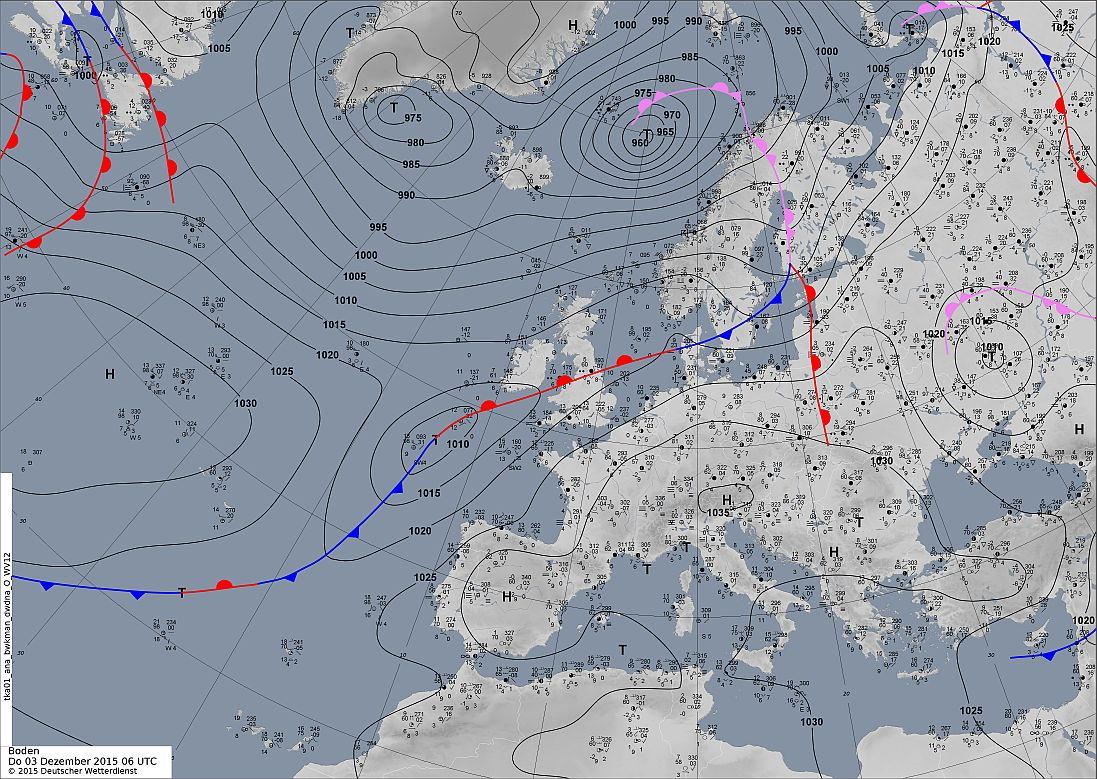
\includegraphics[width=\linewidth]{images/contour-map.jpg}
\caption{Example of a contour map taken from the German Weather Agency (Deutscher Wetter Dienst)~\cite{dwd}}
\label{fig:contour map}
\centering
\end{figure}

Another algorithm, which leverages contour mapping to generate maps of
environmental phenomenons, is a paper by Solis et
al.~\cite{solis2005efficient}. Similiar to the work of Meng et al., the
algorithm suppresses the reporting of readings at nodes which are in the same
isocluster, i.e. there is no isoline between them. An example is given in
Fig.~\ref{fig:contour map}. The space between isolines is dependant on the
application. Less space equals a higher data resolution, as more potential
isolines are between nodes, at the expense of energy, as more readings are
communicated. Readings are scheduled from the farthest leaf nodes (in the case
of a tree topology) to the sink node, which makes additional energy
conservation through shutting down the radio, possible. The authors indicate
that additional temporal suppression is applicabble, as sensor nodes may only
report a reading if that reading changed the isocluster. The authors evaluated
their approach in a simulated environment against multiple other approaches,
e.g. an aggregation scheme, in which data is aggregated at parent nodes into
groups and the averages of the groups are sent further down the network. The
other schemes were a centralized exact approach with and without additional
temporal suppression. The authors found their approach outperfoming the other
algorithms in energy savings and accuracy when constructing contour maps from
sensor readings.

A paper by Silberstein et al.~\cite{silberstein2006constraint} presents a
technique, \textit{Conch}, with which redundant reporting can be reduced even
further compared to the two previous presented schemes. The authors argue that
both algorithms do not leverage the relative differences of sensor nodes
values, i.e. when two sensor nodes differ significantly in their readings, but
one reading can always be infered from the other one, no values should be sent.
In \textit{Conch} a sensor node in a network has a set of sensor nodes from
which it receives updates (updaters) and a set of nodes to which it sends
updates to (reporters). A sensor node broadcasts its sensed values to to the
reporters if its new sensed values differs from the old sensed value by some
margin. When a sensor node receives a value from an updater node, it computes
the difference to its own sensed value. If no value is received, the sensor
node assumes no change has taken place. The base station monitors all
differences between sensor nodes (called edges by the authors), so in the
initialization all reporters send their edges to the base station. Some nodes
are monitored directly and route their sensed values to the base station. At
every timestep, which derives from a user set sampling frequency, the
base station receives updated differences from reporting nodes and sensed values
from directly monitored nodes. This enables the base station to compute the
value of every sensor node at any timestep, if every node can be reached from a
directly monitored node and the corresponding edges. The authors emphasize that
\textit{Conch} is a monitoring algorithm; routing schemes are still used to
route a report from a sensor node to the base station efficiently. The algorithm
is flexible as the authors present ways to build \textit{Conch plans}, i.e.
monitoring topologies, to focus on minimizing energy consumption or increase
sensor node and message failure resilience. The authors tested their algorithm
in different simulated environments against multiple algorithms, i.a. the
scheme by Meng et al.~\cite{meng2004event}. The authors tested the performance
of \textit{Conch} on, i.a. \acp{SN} with different sensor node densities,
predictable increases of the observed value and outlier detection.
\textit{Conch} outperforms all other schemes in terms of energy consumption at
every test and only the scheme of Meng et al. exhibits similiar energy
consumption levels with increasing sensor density.

% EAST. Algorithm basics. Uses a clustering algorithm in which the sensing area
% is devided dynamically into cells. Cells consist of a coordinator (cluster
% head), member and representative sensor nodes. Member nodes do not send their
% data, representative nodes send their sampled values to the coordinator only
% if 


% \subsection{\catIII}
% \label{sec:catIII}

\section{Related Algorithms}
\label{sec:Related Algorithms}

In this section we will present additional algorithms from the area of
routing~\ref{sec:Routing} and topology control~\ref{sec:Topology Control}. We
will also present possible combinations of algorithms which could inspire
further reseach in the area of data sampling from sensor networks
~\ref{sec:Combination of Algorithms}.

% \subsection{Related Algorithms}
% \label{sec:Other Algorithms}

We decided to include routing and topology control as additional classes of
algorithms in \acp{SN}, because all of the schemes described in the taxonomy
use (e.g.~\cite{padhy2006utility}) or presume
(e.g.~\cite{silberstein2006constraint}) some routing and topology control
scheme. There already exist multiple exhaustive surveys on topology
control~\cite{aziz2013survey, li2013survey} and routing~\cite{al2004routing,
pantazis2013energy, singh2010routing}. We will nevertheless show some examples
of routing and topology control algorithms ...

% Ideas: Introduce the following subsections and why we chose to include
% routing and topology building algorithms into the paper but not into the
% taxonomy. E.g. Many of the algorithms in the taxonomy use or presume routing
% and topology building algorithms. Mainly from an energy consumption point of
% view, tree topologies in which nodes closer to the sink/base station have more
% child nodes (i.e. connections to other sensor for which they route the
% information further up the network) need some kind of aggregation mechanisms,
% or such nodes run out of energy faster than other nodes (if you need to cite
% then~\cite{li2013survey}). This will lead to connectivity issues, as the sink
% node / base station looses connections or to even more energy expenditure, as
% sensor nodes which are further away from the sink have to be used as
% gateways. This could be bypassed by using more powerful nodes closer to the
% sink/base station, however, this would make deployment scenarios more
% expensive and less flexible. Li et al.: The authors distinguish between
% static, mobile and hybrid sensor networks. We focus in our work on static
% sensor networks, but want to point out, that mobile sensor networks are an
% interesting and emerging field. Mobile Sensor networks introduce new
% challanges like ever changing topology and connectivity, ..., but they also
% bring new opportunities, like covering a field with less mobile sensors than
% static ones, embedded sensors in cars... Connectivity algorithms play an
% important role in mobile networks, as new sensor nodes can replace dead
% sensor nodes to retain the coverage level in a sensor network.

% Alternatives:
% Maybe put routing and topology building into one subcategory as they both
% deal with inter node connectivity and communication. Topology building is
% often only an initial challange and once a sensor network is deployed, a
% topology is set. But, clustering can be seen as a topology building scheme,
% too. Routing however plays an important role especially after some nodes
% die etc.

\subsection{Routing}
\label{sec:Routing}

Routing schemes define how data is communicated in a network. In a survey from
2004 on routing protocols, Al-Karaki et al.~\cite{al2004routing} classify
routing into network protocols and routing criteria. Network protocols define,
how communication between nodes in a sensor network is structured. With flat
network routing, all nodes have the same task in the network, mainly sensing
and forwarding data. Hierarchical network routing incorporates schemes, in
which the sensor network is divided into clusters. We presented such a scheme
in our taxonomy with \textit{ASAP}~\cite{gedik2007asap}. In location based
routing, sensor nodes are typically equiped with a GPS
module~\cite{xu2001geography} or can infer their own position on based on the
strength of incoming signals, if a GPS module is too
expensive~\cite{hu2004localization}. Location based routing is especially
useful in mobile sensor networks, in which nodes change their position in the
sensing field frequently and therefore change their
neighbors~\cite{hu2004localization}.

A work py Zou et al.~\cite{zou2004pager} introduces a \textit{stateless},
(sensor nodes do not have to save past routing paths) location-based routing
algorithm, \textit{PAGER-M}, for mobile sensor networks. The algorithm uses
greedy forwarding~\cite{stojmenovic2001loop} to rout sensed data to the next
node on the shortest path to the base station. However, sensor nodes can
sometimes be the closest node to the base station in their local topology (but
still out of range to transmit), even though there exists a shorter path and
thus routing can fail, e.g. Fig.~\ref{fig:shadow nodes}. To handle such cases,
the authors define a scheme which idenfies such nodes. Sensor nodes assign cost
variables to themselves, based on the cost variables of its neighbors. This
ensures that every sensor node has a neighbor with a lower cost variable than
itself, which enables a high-cost-to-low-cost routing if greedy routing fails.
The authors tested their algorihtm against \textit{GPSR}~\cite{karp2000gpsr}
and \textit{AODV}~\cite{perkins2003ad} in a simulated environment with ns-2.
\textit{GPSR} is a stateless routing algorithm which uses greedy routing and
perimeter routing when greedy routing fails. Perimeter routing uses the
right-hand rule to traverse a graph couter-clockwise. AODV is a routing
algorithm in which sensor nodes maintain routing paths to frequently
communicated sensor nodes. If no path is known pathfinding is initiated by
broadcasting a route request message. \textit{PAGER-M} outperformed the other
algorithms in package delivery ratio, as the algorithm uses a conservative path
choosing, i.e. a longer routing path is chosen, if a sensor node on the shorter
path is moving aways thus increasing package loss probability. \textit{GPSR}
found the shortest paths on average in the experiment, when sensor nodes had
lower communication ranges. However, the routing overhead and energy
consumption where consistently higher with \textit{GPSR} compared to
\textit{PAGER-M}.

\begin{figure}[h]
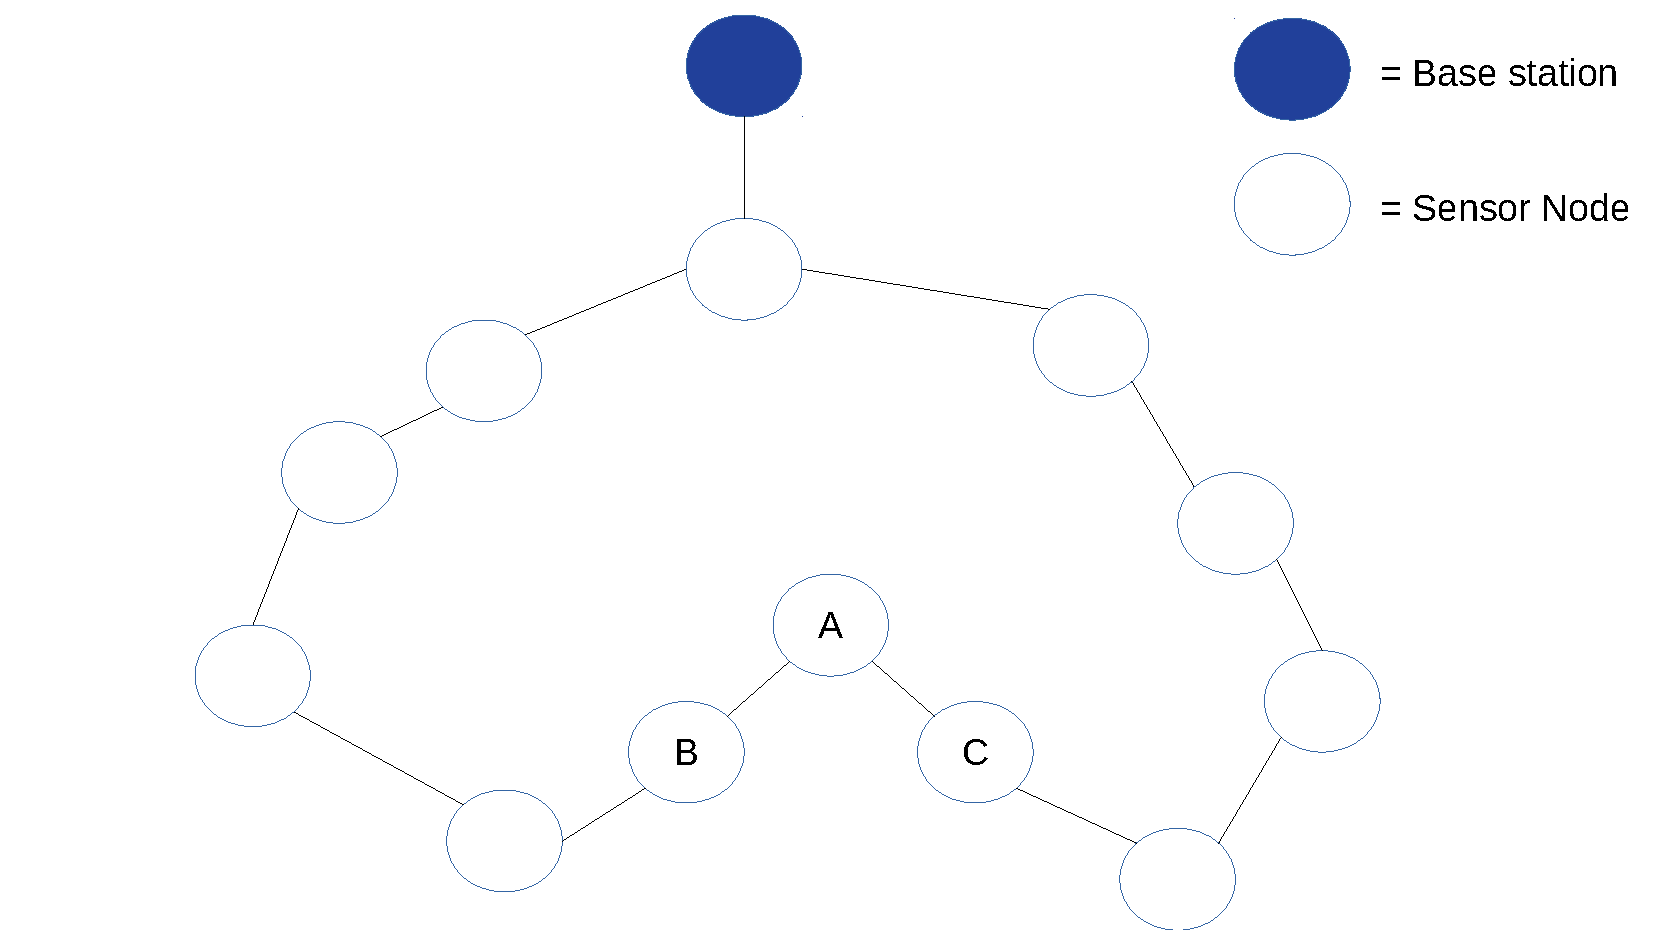
\includegraphics[width=\linewidth]{images/pager-shadow-nodes.pdf}
\caption{Example of a topology where greedy routing can fail. Sensor node A is
the closest node to the base station in its local topology~\cite{zou2004pager}.}
\label{fig:shadow nodes}
\centering
\end{figure}

Pantazis et al. extend the work of Al-Karaki et al. in their survey on routing
protocols~\cite{pantazis2013energy}, with, i.a., Mobile Agent-based protocols.
Such protocols use mobile agents, i.e. software, to visit sensor nodes and
perform tasks, therefore making the \ac{SN} more flexible. Chen et
al.~\cite{chen2007applications}, i.a. justify Mobile Agent-based protocols as a
means to run multiple applications on the same \ac{SN}. As it is unfeasible to
store all application specific programs at each sensor node (due to resource
constraints), mobile agents can be used to migrate between sensor nodes and
perform application specific tasks autonomously.

Chen et al. present multiple algorithms for mobile agent-based protocols in
their work~\cite{chen2011itinerary}. The authors expand with their algorithms
the \textit{LCF} algorithm by Qi et al.~\cite{qi2001optimal}. \textit{LCF}
calculates an ad-hoc itinerary (application specififed route through sensor
nodes) by searching for the closest sensor node to a current node. Chen et al.
expand the algorithm by presenting a scheme to select the first sensor node in
the itinerary which would minize the energy expenditure of the mobile agent.
The authors further propose an algorithm to iteratively optimize the next $ k $
hops of the mobile agent. The authors find in their experiments, in which they
simulate a large-scale \ac{SN} with 800 sensor nodes, that their algorihtm
decreases the energy-delay product ($ energy \cdot delay $) by 80\% in the first
iteration and only marginally in following iterations.

Singh et al.~\cite{singh2010routing} additionally define single-path and
multi-path routing. With single-path routing, sensor nodes send their sensed
values on the shortest path to the base station. With multi-path routing on the
other hand, sensor nodes divide their sensed data and send it with the
\textit{k} shortest paths to the base station. The authors additionally define
different instances of multi-path routing, e.g. disjoint paths and braided
paths. With disjoint paths each path has unique sensor nodes, while in braided
paths a primary path is built and additional paths are computed by excluding
one sensor node from the primary path.

Chen et al.~\cite{chen2011itinerary} present an algorithm, \ac{DGR}, for
routing real-time video data over multiple paths in a \ac{WSN}. \acp{WSN} which
transmit highly commpressed video streams are also called \acp{VSN}. In
\acp{VSN} only a few sensor nodes are equipped with video capturing devides and
more powerful batteries. The rest of the nodes are do not have such equipment
and only serve as relay nodes. The authors argue that \acp{VSN} are limited in
bandwidth and energy and are additionally susceptible to transmission errors.
The algorithm constructs a application specific number of \textit{disjoint}
paths from a source video sensor node to the sink node. To keep the paths
disjoint, the algorithm may construct routes which have nodes that are further
away from the sink than the source node. Such cases can occure when the node
density is low in the \ac{SN} and the path number is high. The authors argue
that disjoint paths are important, as video sent on intersecting paths
"interferes with each other severly". Next hop selection is done in the
algorithm by broadcasting probe messages from the source to the next hop and so
on. A node is selected a the next hop based on its location, i.e. distance to
the \textit{StrategicMappingLocation}, which is a point on the line between the
source node and the sink. The authors tested their algorithm in a simulated
environment with 500 sensor nodes, one video sensor node and one sink against
the already covered \textit{GPSR} with and without additional \ac{FEC}
\footnote{The authors define \ac{FEC} as a scheme which is used to increase
error resilience in real-time video transmission by generating redundant
packets.} coding. The authors simulations show that their scheme outperforms
\textit{GPSR} with and without \ac{FEC} coding in terms of $ \eta $. The metric
$ \eta $ is defined by the authors as $ \eta = \frac{lifetime \cdot
PSNR}{delay}$ with $ lifetime $ specifying the time until the first sensor
nodes dies, $ PSNR $ as peak signal-to-noise ration, i.e. the recieved video
quality, and $ delay $ denoting the "average delay for real-time video
applications".

% are relevant for large scale multihop sensor networks,
% as data is not sent directly from a sensor node to the sink, but routed through
% some intermediary sensor nodes. This is because sending messages directly does
% not scale well with increasing number of sensor nodes in terms of energy
% expenditure~\cite{padhy2006utility}. In addition, finding optimal routing paths
% in \acp{SN} in which sensor nodes may fail or additional aggregation has to
% take place during hops, is not trivial.

% Insights Al-Karaki et al.: Different node deployment options: Manual and
% random. With manual placement, routing paths can be planned, while random
% deployment requires routing paths to be formed ad hoc. The authors define
% routing protocols similiar to Aziz et al. and Li et al. defining topology
% building protocols. The authors include in network aggregation in their
% routing taxonomy. A lot of routing algorithms presented in the survey, deal
% with the diffusion of user queries; mainly based on directed diffusion.
% Clustering is also included in the survey, which is kind of a topology
% building technique. Their work deals with network structure and protocol
% operation. Network structure deals with how routes are found, i.e. flat
% routing -> sensor nodes send their values to the next neighbor/parent,
% hierarchical network routing -> sensor nodes are grouped into clusters,
% location based routing -> sensor nodes can identify their own coordinates and
% the coordinates of other nodes, which is especially useful in mobile sensor
% networks, as sensor nodes change their location. Protocol operation deals
% with on which premise routes are build, i.e. the route with the highes
% quality of service is found or a query optimizer decides how to best execute
% an imperative user statement.

% Insights Singh et al.: The categorization of routing protocols is similiar to
% Al-Karaki et al. They define single-path routing and multi-path routing.
% Single path -> a sensor node sends its data to the sink via the shortest
% route. Multi-path -> A sensor node finds the k shortest paths to the sink
% node and divides its data to "tax" the paths evenly. Maybe take some pictures
% from the paper.

% Insights Pantazis et al.: The paper extends the taxonomy presented by
% Al-Karaki et al. The paper is really long with a lot of sources. The authors
% have a subcategory, "Topology Based", in their taxonomy. So this basically
% set the nail in the coffin of making two distinct categories here. The
% authors Topology category deals with the location of the nodes.

\subsection{Topology Control}
\label{sec:Topology Control}

% Insights Aziz et al.: There are a lot of definitions of network
% liftime~\cite{aziz2013survey}. Aziz et al. include algorithms in their work
% for a survey on topology building routing algorithms. So it is possible, that
% topology building (or topology control) and routing are the same. The authors
% say that topology building can be done through varying transmission power to,
% i.e. not communicating to a sink directly, but sending it to other nodes in a
% multihop fashion. Li et al. also present this problem as finding the minimum
% transmission power with which connectivity is still warranted. Additionally,
% sensor nodes can have different and dynamic transmission power settings or
% can be configured to all have the same transmission power setting. Another
% technique the authors bring up is basically duty cycling, i.e. putting a
% sensor node into sleep, idle, listening, transmit mode. The third technique
% is clustering. The fourth technique is a hybrid technique which utilizes some
% sort of clustering algorithm and schemes from the previous techniques.

% Insights Li et al.~\cite{li2013survey}: Coverage and connectivity are the
% main aspects topology control deals with. Network Coverage is defined by the
% authors as "how well the target field is monitored by the sensor network".
% This affects where sensor nodes are placed, e.g. if sensing ranges overlap or
% cover the whole field, then the network has blanket coverage. Connectivity
% deals with how well and to what costs sensor nodes in a network can
% communicate with each other. Similiar to Aziz et al.~\cite{aziz2013survey},
% the authors bring up duty cycling and route building as techniques for
% handling network connectivity. Duty cycling in combination with network
% coverage is present in the work of Tian et al., (CITE AND REREAD THAT) where
% sensor nodes go into sleep mode when the area they are sensing is already
% covered enough by neighbor sensor nodes. They also define additional high
% level use cases for sensor networks, i.e. monitoring an area, a breach of an
% area or some points of interest (POI). They bring up the point, that in
% network topology design, a tradeoff between network performance, i.e. network
% coverage, data quality, and network lifetime, i.e. network connectivity, is
% given. The authors point out, that real life deployments of wireless sensor
% networks are providing multiple network services. To stay efficient and be
% scalable, protocols have to support multiple network services. If a system
% integrates multiple protocols for the multiple network services, the
% complexity of such a system can have negative impact on scalability and
% efficiency. THIS CAN BE A GOOD INTRODUCTION TO COMBINATION OF ALGORITHMS.

Topology Control is defined by Aziz et al.~\cite{aziz2013survey} as "a
technique that uses any controlled network parameter to generate and maintain a
topology for the benefits of reducing energy consumption and achieving a
desired property for an entire network." Modifiable parameters are listed by
the authors as transmission power of the radio, changing the mode of sensor
nodes and clustering. Sensor nodes can manipulate the transmission power of
their radios to vary the transmission range and therefore reduce energy
expenditure for communication. While clustering is also mentioned as a
\textit{routing} technique, changing modes of sensor nodes is a new
classification, also called \textit{duty cycling}~\cite{carrano2014survey,
lin2004medium, buettner2006x}. As Carrano et al. point
out~\cite{carrano2014survey}, duty cycling finds a tradeoff between latency and
energy consumption in \acp{SN}. End-to-end latency increases, if routing sensor
nodes have to wait for the next sensor node in the routing path to wake up.
Additionally, the authors argue, that although a sensor node consumes less
energy in sleep mode, i.e. the radio transceiver is turned off, higher data
collision rates and potential control packet overhead, induced by duty cycling,
can increase energy expenditure.

Sun et al.~\cite{sun2008ri} present a \ac{MAC} protocol which tackles the
aforementioned problems. With the protocol \textit{RI-MAC} every sensor node
has a wake up schedule. While awake, a sensor node will broadcast a message
that it is ready to receive data. A sender node, which is awake and waiting for
the message, then starts data transmission, which the receiving node
acknowledges. The authors argue, that due to the receiver initiated
transmission, \textit{RI-MAC} handles heavier traffic loads more power
efficiently, than other \ac{MAC} protocols, such as \textit{B-MAC} and
\textit{X-MAC}. This is because the broadcasted message by a receiver sensor
node has a backoff window size with which the receiver can schedule different
sender nodes. The authors tested their protocol extensively on a small, real
world testbed and in a large \ac{SN} simulated with the ns-2
tool~\cite{bajaj1999improving}. Their tests were additionally run on
\textit{X-MAC}~\cite{buettner2006x}, in which data transmission is not
initiated by the receiver, and \textit{X-MAC-UMPA} which is a simplification of
\textit{X-MAC}. In both test environments, \textit{RI-MAC} outperformed the
other two algorithms in, i.a. average packet delivery ratio and average
latency.

Li et al.~\cite{li2013survey} address in their survey on topology control,
network coverage as a key issue in \acp{SN}. Network coverage is defined by the
authors as "the surveillance map of the target field, which emphasizes the
sensors' placement positions and cooperations among sensors". A target field
has observable points and can be covered by sensor nodes to monitor every point
in the field. The authors define such coverage as blanket coverage. Barrier
coverage is a type of topology where the sensor nodes are laid-out in such a
way, that the outlines of a field are monitored. Liu et
al.~\cite{liu2008strong} define a barrier as "the union of the covered areas of
sensors". Barrier coverage can be used to spot intruders, if they cross an area
covered by a sensor node. However, barrier coverages can have gaps (e.g.
Fig.~\ref{fig:coverage}), especially if the sensor nodes are deployed randomly,
e.g. dropped from an airplane, and have scheduling mechanisms to turn off their
sensors~\cite{liu2008strong}. The algorithm devides the observed area into
smaller regions. Each region is devided into disjoint segments, where sensor
nodes are distributed horizontally, and vertical strip, where sensor nodes are
distributed vertically. Afterwards, the algorithm computes how many disjoint
segments need to be active to provide full barrier coverage with no gaps.
Through rotation of the active segments, a longer network lifetime can be
achieved. The authors tested their approach in a simulated environment against
a centralized approach, i.e. barriers are computed for the whole area. The
authors found that their algorithm forms stronger barriers, i.e. more local
barriers are found in the segments than in the whole area. Additionally, the
authors argue that their algorithm has lower communication overhead and
computational costs than the centralized algorithm, because sensor nodes only
have to communicate in their local segments.

% TODO Potentielly add 3D sensor networks and Sweep Coverage

\begin{figure}
\begin{subfigure}{.5\textwidth}
  \centering
  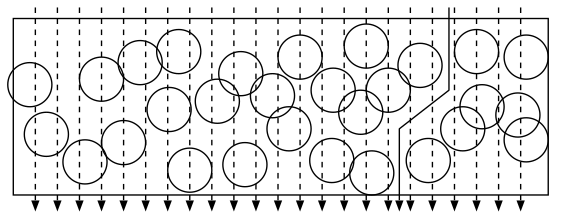
\includegraphics[width=.8\linewidth]{images/weak-coverage.png}
  \caption{}
  \label{fig:weak}
\end{subfigure}%
\begin{subfigure}{.5\textwidth}
  \centering
  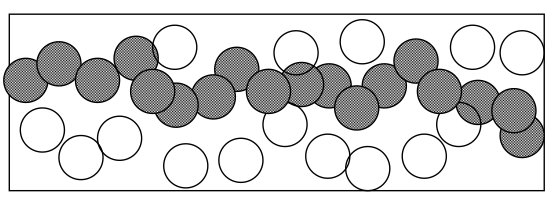
\includegraphics[width=.8\linewidth]{images/strong-coverage.png}
  \caption{}
  \label{fig:strong}
\end{subfigure}
\caption{Example of a weak (a) and a strong (b) barrier coverage \ac{SN}}
\label{fig:coverage}
\end{figure}

\FloatBarrier

% What to look out for: What is topology building? Are algorithms which are
% classified as topology building algorithms, only used once in a sensor
% network, i.e. when the network is set up a routing topology is created? Use
% cases for those algorithms -> node failure handling, i.e. connections between
% nodes have to be reestablished, mobile nodes, i.e. connectivity changes
% continuosly... Another important aspect is the interaction between topology
% building and routing. Which aspects differentiate them from each other? Are
% there even any differences in routing and topology building?

\subsection{Combination of Algorithms}
\label{sec:Combination of Algorithms}
% I decided to include Adam and Admin as an example of combination of
% algorithms as it is a framework which has filtering and sampling techniques
% additionally, in the experiments the authors compared their framework i.a.
% against L-SIP which is a model based scheme
A more recent paper from Trihinas et al.~\cite{trihinas2015adam} provides
framework for finding a sampling rate which optimizes the tradeoff between
energy consumption and quality of data. The framework was implemented in java
with no external dependencies. The algorithm estimates a metric stream $ M $ to
reduce the number of sampling periods when the metric stream does not fluctuate
and vice versa. A sampling period $ T_i $ is computed by estimating the metric
stream evolution. The authors use a \ac{PEWMA} to produce an estimated metric
stream $ M' $. The \ac{PEWMA} is a Variation of \ac{EWMA} which provides a
one-step ahead estimation. The authors state that \ac{PEWMA} is more robust
against abrunt transient changes in the metric evoultion than \ac{EWMA}.

When $ M' $ differs from $ M $ by a user specified imprecision value $
\gamma $, then $ T_i $ is increased to a maximum sampling period $ T_{max}
$. Otherwise $ T_i $ is decreased to a minimal sampling period $ T_{min}
$. The algorithm was tested against \ac{EWMA}, L-SIP and FAST. L-SIP is a  

% Further Possible combinations: 

% The authors of \textit{Conch} argue that their in-network suppression
% algorithm can be integrated into model based schemes such as the one
% of~\cite{jain2004adaptive}. \textit{Backcasting} can be combined with the
% cluster head cycling algorithm of ASAP. EDAL combines routing techniques with
% compressive sampling.

\section{Conclusion}

% Some general thoughts on disadvantages in compressed sampling. Beside the
% obvious assumptions of data or a signal being sparse in a domain or having
% short-term stability or other features, the above mentioned algorithms (CDG,
% EDCA, STCDG) do not offer a (smart) way of dealing with outliers. STCDG just
% sends those values to the sink. Furthermore, sensing/sampling costs are not
% included in power consumption analysis